\documentclass[11pt]{article}
\usepackage[utf8]{inputenc}
\usepackage[T1]{fontenc}
\usepackage[margin=1in]{geometry}
\usepackage{amsmath,amssymb}
\usepackage{graphicx}
\usepackage{booktabs}
\usepackage{listings}
\usepackage{xcolor}
\usepackage{array}
\usepackage[hidelinks]{hyperref}
\lstset{basicstyle=\footnotesize\ttfamily, columns=fullflexible, breaklines=true, keepspaces=true}
% generated by gen_numbers.py -- do not edit
\newcommand{\dOneOm}{0.2939}
\newcommand{\dOneHrd}{101.94}
\newcommand{\dOneChi}{12.74}
\newcommand{\dOneDof}{10}
\newcommand{\dOneGridOm}{0.2957}
\newcommand{\dOneGridHrd}{101.79}
\newcommand{\dOneTOm}{0.295}
\newcommand{\dOneTOmS}{0.015}
\newcommand{\dOneTHrd}{101.8}
\newcommand{\dOneTHrdS}{1.3}
\newcommand{\dOnePullOm}{-0.074}
\newcommand{\dOnePullHrd}{0.105}
\newcommand{\dOneAbsPullOm}{0.074}
\newcommand{\dOneAbsPullHrd}{0.105}
\newcommand{\dOneSource}{DESI DR1 2024 VI, arXiv:2404.03002, quoted from fetched paper text}
\newcommand{\dOneNdata}{12}
\newcommand{\dTwoLOm}{0.29781}
\newcommand{\dTwoLOmS}{0.00856}
\newcommand{\dTwoLOmT}{0.2975}
\newcommand{\dTwoLOmTS}{0.0086}
\newcommand{\dTwoLOmP}{0.037}
\newcommand{\dTwoLOmW}{0.995}
\newcommand{\dTwoLOmG}{0.29783}
\newcommand{\dTwoLHrd}{101.530}
\newcommand{\dTwoLHrdS}{0.732}
\newcommand{\dTwoLHrdT}{101.54}
\newcommand{\dTwoLHrdTS}{0.73}
\newcommand{\dTwoLHrdP}{-0.013}
\newcommand{\dTwoLHrdW}{1.003}
\newcommand{\dTwoLHrdG}{101.523}
\newcommand{\dTwoWOm}{0.29713}
\newcommand{\dTwoWOmS}{0.00896}
\newcommand{\dTwoWOmT}{0.2969}
\newcommand{\dTwoWOmTS}{0.0089}
\newcommand{\dTwoWOmP}{0.026}
\newcommand{\dTwoWOmW}{1.007}
\newcommand{\dTwoWOmG}{0.29714}
\newcommand{\dTwoWw}{-0.9164}
\newcommand{\dTwoWwS}{0.0787}
\newcommand{\dTwoWwT}{-0.916}
\newcommand{\dTwoWwTS}{0.078}
\newcommand{\dTwoWwP}{-0.005}
\newcommand{\dTwoWwW}{1.009}
\newcommand{\dTwoWwG}{-0.9170}
\newcommand{\dTwoMaxAbsPull}{0.037}
\newcommand{\dTwoWHrd}{99.83}
\newcommand{\dTwoWHrdS}{1.73}
\newcommand{\dTwoCorr}{-0.923}
\newcommand{\dTwoCorrT}{-0.92}
\newcommand{\dTwoChi}{10.27}
\newcommand{\dTwoDof}{11}
\newcommand{\dTwoBestOm}{0.29746}
\newcommand{\dTwoBestHrd}{101.540}
\newcommand{\dTwoFishOmS}{0.00858}
\newcommand{\dTwoFishHrdS}{0.733}
\newcommand{\dTwoEmceeGrid}{0.009}
\newcommand{\dTwoCritPass}{14}
\newcommand{\dTwoCritN}{14}
\newcommand{\dTwoNsteps}{20000}
\newcommand{\dTwoIOm}{0.29498}
\newcommand{\dTwoIOmP}{-0.001}
\newcommand{\dTwoIHrd}{101.89}
\newcommand{\dTwoIHrdP}{0.067}
\newcommand{\shOmOne}{0.29498}
\newcommand{\shOmTwo}{0.29781}
\newcommand{\shDelta}{0.00283}
\newcommand{\shPub}{0.0025}
\newcommand{\shSigNestOwn}{0.01194}
\newcommand{\shSigNestPre}{0.01229}
\newcommand{\shSigInd}{0.01700}
\newcommand{\shRatioOwn}{0.237}
\newcommand{\shRatioPre}{0.231}
\newcommand{\shRatioInd}{0.167}
\newcommand{\shDhrd}{-0.356}
\newcommand{\dTwoRadOm}{-0.046}
\newcommand{\dTwoRadHrd}{0.013}
\newcommand{\dTwoCambOm}{0.032}
\newcommand{\dTwoCambHrd}{-0.011}
\newcommand{\dTwoCambMassless}{2.3\times10^{-11}}
\newcommand{\dTwoNPC}{5}
\newcommand{\dTwoNPCkeys}{6}
\newcommand{\dTwoNNC}{5}
\newcommand{\dTwoPCpullStdOm}{0.970}
\newcommand{\dTwoPCpullMeanOm}{-0.002}
\newcommand{\dTwoPCn}{500}
\newcommand{\dTwoNCfiveMed}{3.4\times10^{-6}}
\newcommand{\dTwoNCfiveBad}{6}
\newcommand{\dTwoNCfiveN}{20}
\newcommand{\dTwoNCthreeChi}{1420.2}
\newcommand{\dTwoRefN}{8}
\newcommand{\dTwoRefVerdict}{minor}
\newcommand{\dTwoRerunIdentical}{yes}
\newcommand{\hzPOne}{68.545}
\newcommand{\hzPOneS}{0.594}
\newcommand{\hzPOneOm}{0.2977}
\newcommand{\hzPOneOmS}{0.0085}
\newcommand{\hzPOneD}{0.035}
\newcommand{\hzPOneP}{0.060}
\newcommand{\hzPOneOmP}{-0.001}
\newcommand{\hzPOneR}{1.024}
\newcommand{\hzPOneV}{PASS}
\newcommand{\hzPTwo}{68.697}
\newcommand{\hzPTwoS}{0.809}
\newcommand{\hzPTwoOm}{0.2953}
\newcommand{\hzPTwoOmS}{0.0146}
\newcommand{\hzPTwoD}{0.167}
\newcommand{\hzPTwoP}{0.209}
\newcommand{\hzPTwoOmP}{0.022}
\newcommand{\hzPTwoR}{1.012}
\newcommand{\hzPTwoV}{PARTIAL}
\newcommand{\hzSOne}{68.579}
\newcommand{\hzSOneS}{0.601}
\newcommand{\hzSOneOm}{0.2976}
\newcommand{\hzSOneOmS}{0.0086}
\newcommand{\hzSOneD}{0.069}
\newcommand{\hzSOneP}{0.119}
\newcommand{\hzSOneOmP}{-0.015}
\newcommand{\hzSOneR}{1.037}
\newcommand{\hzSOneV}{PASS}
\newcommand{\hzSTwo}{68.701}
\newcommand{\hzSTwoS}{0.815}
\newcommand{\hzSTwoOm}{0.2946}
\newcommand{\hzSTwoOmS}{0.0143}
\newcommand{\hzSTwoD}{0.171}
\newcommand{\hzSTwoP}{0.214}
\newcommand{\hzSTwoOmP}{-0.028}
\newcommand{\hzSTwoR}{1.018}
\newcommand{\hzSTwoV}{PARTIAL}
\newcommand{\hzTOne}{68.51}
\newcommand{\hzTOneS}{0.58}
\newcommand{\hzTTwo}{68.53}
\newcommand{\hzTTwoS}{0.80}
\newcommand{\hzTOneb}{0.2977}
\newcommand{\hzTOnebS}{0.0086}
\newcommand{\hzTTwob}{0.295}
\newcommand{\hzTTwobS}{0.015}
\newcommand{\hzStrict}{0.15}
\newcommand{\hzSoft}{0.33}
\newcommand{\hzStrictSigOne}{0.26}
\newcommand{\hzStrictSigTwo}{0.19}
\newcommand{\hzPsuccess}{0.55}
\newcommand{\hzPsuccessOr}{0.80}
\newcommand{\hzBBNob}{0.02218}
\newcommand{\hzBBNobS}{0.00055}
\newcommand{\hzPreTime}{2026-09-27T15:53:42Z}
\newcommand{\hzAmdTime}{2026-09-27T16:04:27Z}
\newcommand{\hzLockShaShort}{b7fe5608e4ae6d0b}
\newcommand{\hzLockWritten}{16:03:03Z}
\newcommand{\hzLockMatch}{yes}
\newcommand{\hzLockShaNowMatches}{yes}
\newcommand{\hzLockOne}{68.579}
\newcommand{\hzLockOneS}{0.601}
\newcommand{\hzLockTwo}{68.701}
\newcommand{\hzLockTwoS}{0.815}
\newcommand{\hzLockDiff}{0.0}
\newcommand{\hzPmSOne}{-0.034}
\newcommand{\hzPmSTwo}{-0.0044}
\newcommand{\hzProxySys}{0.139}
\newcommand{\hzAubCambMaxPct}{0.029}
\newcommand{\hzGOnePullOm}{0.024}
\newcommand{\hzGOnePullHrd}{-0.027}
\newcommand{\hzGTwoPullOm}{-0.033}
\newcommand{\hzGTwoPullHrd}{0.103}
\newcommand{\hzTTwoMargin}{0.017}
\newcommand{\hzTTwoMC}{0.014}
\newcommand{\hzPostHocEight}{0.183}
\newcommand{\hzPostHocSix}{0.046}
\newcommand{\hzRebudget}{0.050}
\newcommand{\hzHrdQuoteEight}{101.8}
\newcommand{\hzHrdQuoteSix}{101.9}
\newcommand{\hzOmTol}{0.25}
\newcommand{\hzPtwoN}{100}
\newcommand{\hzCambAnchor}{147.049}
\newcommand{\hzCambAnchorPre}{147.049}
\newcommand{\hzNfourD}{0.164}
\newcommand{\hzNfourMargin}{0.014}
\newcommand{\hzNfourMarginSig}{0.02}
\newcommand{\hzMnu}{0.06}
\newcommand{\hzNfourChi}{-5.2\times10^{-5}}
\newcommand{\hzNfourStatus}{post-hoc (referee fix round), not preregistered, not in the verdict's controls condition}
\newcommand{\hzPoneD}{0.0041}
\newcommand{\hzPtwoMean}{-0.064}
\newcommand{\hzPtwoStd}{1.023}
\newcommand{\hzNthree}{21.0}
\newcommand{\hzNtwoChi}{1420.2}
\newcommand{\hzPfour}{1.7\times10^{-6}}
\newcommand{\hzRefN}{8}
\newcommand{\hzRefVerdict}{minor}
\newcommand{\hzRowav}{68.545}
\newcommand{\hzRowas}{0.594}
\newcommand{\hzRowat}{68.51}
\newcommand{\hzRowats}{0.58}
\newcommand{\hzRowap}{0.060}
\newcommand{\hzRowbv}{0.2977}
\newcommand{\hzRowbs}{0.0085}
\newcommand{\hzRowbt}{0.2977}
\newcommand{\hzRowbts}{0.0086}
\newcommand{\hzRowbp}{-0.001}
\newcommand{\hzRowcv}{68.697}
\newcommand{\hzRowcs}{0.809}
\newcommand{\hzRowct}{68.53}
\newcommand{\hzRowcts}{0.80}
\newcommand{\hzRowcp}{0.209}
\newcommand{\hzRowdv}{0.2953}
\newcommand{\hzRowds}{0.0146}
\newcommand{\hzRowdt}{0.295}
\newcommand{\hzRowdts}{0.015}
\newcommand{\hzRowdp}{0.022}
\newcommand{\hzRowev}{68.579}
\newcommand{\hzRowes}{0.601}
\newcommand{\hzRowet}{68.51}
\newcommand{\hzRowets}{0.58}
\newcommand{\hzRowep}{0.119}
\newcommand{\hzRowfv}{0.2976}
\newcommand{\hzRowfs}{0.0086}
\newcommand{\hzRowft}{0.2977}
\newcommand{\hzRowfts}{0.0086}
\newcommand{\hzRowfp}{-0.015}
\newcommand{\hzRowgv}{68.701}
\newcommand{\hzRowgs}{0.815}
\newcommand{\hzRowgt}{68.53}
\newcommand{\hzRowgts}{0.80}
\newcommand{\hzRowgp}{0.214}
\newcommand{\hzRowhv}{0.2946}
\newcommand{\hzRowhs}{0.0143}
\newcommand{\hzRowht}{0.295}
\newcommand{\hzRowhts}{0.015}
\newcommand{\hzRowhp}{-0.028}
\newcommand{\hzRowiv}{101.52}
\newcommand{\hzRowis}{0.74}
\newcommand{\hzRowit}{101.54}
\newcommand{\hzRowits}{0.73}
\newcommand{\hzRowip}{-0.027}
\newcommand{\hzRowjv}{0.2977}
\newcommand{\hzRowjs}{0.0087}
\newcommand{\hzRowjt}{0.2975}
\newcommand{\hzRowjts}{0.0086}
\newcommand{\hzRowjp}{0.024}
\newcommand{\hzRowkv}{101.93}
\newcommand{\hzRowks}{1.27}
\newcommand{\hzRowkt}{101.80}
\newcommand{\hzRowkts}{1.30}
\newcommand{\hzRowkp}{0.103}
\newcommand{\hzRowlv}{0.2945}
\newcommand{\hzRowls}{0.0145}
\newcommand{\hzRowlt}{0.295}
\newcommand{\hzRowlts}{0.015}
\newcommand{\hzRowlp}{-0.033}
\newcommand{\ebSOm}{0.2987}
\newcommand{\ebSOmS}{0.0164}
\newcommand{\ebSOmT}{0.299}
\newcommand{\ebSOmTS}{0.016}
\newcommand{\ebSOmP}{-0.017}
\newcommand{\ebSHrd}{100.52}
\newcommand{\ebSHrdS}{1.29}
\newcommand{\ebSHrdT}{100.40}
\newcommand{\ebSHrdTS}{1.30}
\newcommand{\ebSHrdP}{0.090}
\newcommand{\ebDOm}{0.2980}
\newcommand{\ebDOmS}{0.0087}
\newcommand{\ebDOmT}{0.2975}
\newcommand{\ebDOmTS}{0.0086}
\newcommand{\ebDOmP}{0.055}
\newcommand{\ebDHrd}{101.51}
\newcommand{\ebDHrdS}{0.75}
\newcommand{\ebDHrdT}{101.54}
\newcommand{\ebDHrdTS}{0.73}
\newcommand{\ebDHrdP}{-0.043}
\newcommand{\ebChi}{1.93}
\newcommand{\ebPTE}{0.381}
\newcommand{\ebNsig}{0.877}
\newcommand{\ebNsigGrid}{0.862}
\newcommand{\ebNsigMAP}{0.932}
\newcommand{\ebNsigGauss}{0.815}
\newcommand{\ebNsigKDE}{0.939}
\newcommand{\ebOneDOm}{0.041}
\newcommand{\ebOneDHrd}{0.668}
\newcommand{\ebSCorr}{-0.880}
\newcommand{\ebBaseVsGauss}{0.032}
\newcommand{\ebLitLo}{0.32}
\newcommand{\ebLitHi}{1.56}
\newcommand{\ebTol}{0.5}
\newcommand{\ebInjN}{12.1}
\newcommand{\ebInjScale}{0.93}
\newcommand{\ebEdsGauss}{376.4}
\newcommand{\ebPosN}{200}
\newcommand{\ebPosCalFrac}{0.03}
\newcommand{\ebRefOneN}{7}
\newcommand{\ebRefTwoN}{9}
\newcommand{\ebFixOneFixed}{8}
\newcommand{\ebFixOneN}{9}
\newcommand{\ebFixTwoFixed}{7}
\newcommand{\ebFixTwoN}{10}
\newcommand{\rsCvOm}{0.29743}
\newcommand{\rsCvOmS}{0.00861}
\newcommand{\rsCvHrd}{101.543}
\newcommand{\rsCvHrdS}{0.735}
\newcommand{\rsCvChi}{10.2710}
\newcommand{\rsQdOm}{0.29746}
\newcommand{\rsQdHrd}{101.540}
\newcommand{\rsCvMinusPyOm}{-3.2\times10^{-5}}
\newcommand{\rsQdMinusPyOm}{-1.8\times10^{-6}}
\newcommand{\rsEdsErr}{7.4\times10^{-7}}
\newcommand{\rsAdamsErr}{2.1\times10^{-4}}
\newcommand{\rsTestsPass}{12}
\newcommand{\rsTestsIgn}{1}
\newcommand{\rsPortCommit}{c46a680}
\newcommand{\rsFixCommit}{d22cf01}
\newcommand{\lnAN}{3}
\newcommand{\lnAPA}{3}
\newcommand{\lnARcOne}{0}
\newcommand{\lnATOne}{16.0}
\newcommand{\lnARcTwo}{0}
\newcommand{\lnATTwo}{645.0}
\newcommand{\lnASha}{c85c1e8abe28}
\newcommand{\lnBN}{6}
\newcommand{\lnBPA}{6}
\newcommand{\lnBRcOne}{0}
\newcommand{\lnBTOne}{108.2}
\newcommand{\lnBRcTwo}{1}
\newcommand{\lnBTTwo}{138.0}
\newcommand{\lnBSha}{3b451bd5a93d}
\newcommand{\lnCN}{10}
\newcommand{\lnCPA}{10}
\newcommand{\lnCRcOne}{0}
\newcommand{\lnCTOne}{23.2}
\newcommand{\lnCRcTwo}{0}
\newcommand{\lnCTTwo}{367.6}
\newcommand{\lnCSha}{2b6530838efa}
\newcommand{\lnDN}{9}
\newcommand{\lnDPA}{9}
\newcommand{\lnDRcOne}{0}
\newcommand{\lnDTOne}{10.6}
\newcommand{\lnDRcTwo}{0}
\newcommand{\lnDTTwo}{313.1}
\newcommand{\lnDSha}{560e3b5d8266}
\newcommand{\lnTotal}{28}
\newcommand{\lnTotalJson}{28}
\newcommand{\lnCleanOne}{28}
\newcommand{\lnCleanTwo}{22}
\newcommand{\lnBlockedTwo}{6}
\newcommand{\lnPairs}{7}
\newcommand{\lnPairsTotal}{8}
\newcommand{\lnNegRcOne}{0}
\newcommand{\lnNegRcTwo}{0}
\newcommand{\lnNegTOne}{8.3}
\newcommand{\lnNegTTwo}{162.0}
\newcommand{\lnNegSorry}{yes}
\newcommand{\lnAxRcOne}{0}
\newcommand{\lnAxRcTwo}{0}
\newcommand{\lnAxSeen}{yes}
\newcommand{\lnAxRejected}{yes}
\newcommand{\lnToolchain}{leanprover/lean4:v4.34.0-rc2}
\newcommand{\lnMathlibRev}{85e3a25e006c}
\newcommand{\lnMathlibInput}{v4.34.0-rc2}
\newcommand{\lnLeanVersion}{4.34.0-rc2}
\newcommand{\lnLoad}{4.34 / 4.42 / 4.84}
\newcommand{\lnVoneSha}{bc09047fb601}
\newcommand{\lABound}{0}
\newcommand{\lAN}{6}
\newcommand{\lATA}{3}
\newcommand{\lATB}{1}
\newcommand{\lATL}{2}
\newcommand{\lATC}{0}
\newcommand{\lAAud}{0}
\newcommand{\lARc}{1}
\newcommand{\lBBound}{6}
\newcommand{\lBN}{25}
\newcommand{\lBTA}{6}
\newcommand{\lBTB}{8}
\newcommand{\lBTL}{10}
\newcommand{\lBTC}{1}
\newcommand{\lBAud}{6}
\newcommand{\lBRc}{0}
\newcommand{\lCBound}{0}
\newcommand{\lCN}{43}
\newcommand{\lCTA}{10}
\newcommand{\lCTB}{17}
\newcommand{\lCTL}{15}
\newcommand{\lCTC}{1}
\newcommand{\lCAud}{8}
\newcommand{\lCRc}{1}
\newcommand{\lDBound}{0}
\newcommand{\lDN}{27}
\newcommand{\lDTA}{9}
\newcommand{\lDTB}{8}
\newcommand{\lDTL}{8}
\newcommand{\lDTC}{2}
\newcommand{\lDAud}{9}
\newcommand{\lDRc}{0}
\newcommand{\rgSlope}{0.49}
\newcommand{\rgGOneMax}{0.25}
\newcommand{\rgGTwoMax}{0.45}
\newcommand{\rgGOneOff}{-0.020}
\newcommand{\rgGOneOffH}{-0.027}
\newcommand{\rgGTwoOff}{0.134}
\newcommand{\rgGTwoOffP}{0.10}
\newcommand{\rgGTwoOffH}{0.183}
\newcommand{\rgGTwoPassed}{passed}
\newcommand{\rcSigCone}{0.0061}
\newcommand{\rcRatioCone}{0.46}
\newcommand{\roNsigFiftySeven}{1.34}
\newcommand{\roPTEFiftySeven}{0.18}
\newcommand{\rnMC}{0.0107}
\newcommand{\rnRatio}{1.3}
\newcommand{\rpCambPull}{0.005}
\newcommand{\rpRadPull}{-0.009}
\newcommand{\rmDRtwoMC}{0.007}
\newcommand{\raNexceed}{2}
\newcommand{\raNpts}{5}
\newcommand{\raWorstOb}{0.02218}
\newcommand{\raWorstOc}{0.119}
\newcommand{\rsPRMerge}{7c9c3c3}
\newcommand{\rsPRMergedAt}{2026-09-27T17:29:02Z}
\newcommand{\rbAudited}{8}
\newcommand{\rbSame}{8}
\newcommand{\rbAuditSha}{c0663994}
\newcommand{\rbCurSha}{2b653083}
\newcommand{\rdPubChi}{12.66}
\newcommand{\rdPubOm}{0.294}
\newcommand{\rdPubHrd}{101.94}
\newcommand{\rdMzero}{0.081}
\newcommand{\rdMaxChange}{0.003}
\newcommand{\rdMthree}{0.078}
\newcommand{\mtMtwo}{0/0}
\newcommand{\mtMfour}{0/0}
\newcommand{\rtLo}{0.11}
\newcommand{\rtHi}{0.25}
\newcommand{\rtMin}{0.05}
\newcommand{\rtMax}{0.25}
\newcommand{\rtMChrd}{0.028}
\newcommand{\rtMCH}{0.038}
\newcommand{\rtGtwoSteps}{2000}
\newcommand{\rtGtwoESS}{2115}
\newcommand{\rtDesiMC}{0.025}
\newcommand{\rtComb}{0.029}
\newcommand{\rtMarginComb}{0.58}
\newcommand{\raNexceedSix}{1}
\newcommand{\raMaxSixPct}{0.0224}
\newcommand{\raShiftLo}{6.7}
\newcommand{\raShiftHi}{6.9}
\newcommand{\raEqSeventeen}{6.5}
\newcommand{\raCambVer}{2.0.4}
\newcommand{\rgStepOm}{0.00143}
\newcommand{\rgStepHrd}{0.179}
\newcommand{\rgNgrid}{141}
\newcommand{\rgNodesOm}{1.3}
\newcommand{\rgNodesHrd}{0.8}
\newcommand{\rgGridChi}{12.7562}
\newcommand{\hzPtwoOmMean}{-0.131}
\newcommand{\hzPtwoOmStd}{0.944}
\newcommand{\hzPtwoOmSE}{0.094}
\newcommand{\zgRc}{0}
\newcommand{\zgSha}{ca31d646}
\newcommand{\mbOne}{3431}
\newcommand{\mbTwo}{8370}
\newcommand{\mbSrc}{8370}
\newcommand{\lrMainFlat}{2}
\newcommand{\lrMainNew}{0}
\newcommand{\evCosPy}{3.11.16}
\newcommand{\evCosNp}{2.4.6}
\newcommand{\evCosSp}{1.17.1}
\newcommand{\evPtaPy}{3.10.12}
\newcommand{\evPtaNp}{1.26.4}
\newcommand{\evPtaSp}{1.15.3}
\newcommand{\evEmcee}{3.1.6}
\newcommand{\reCosNdiff}{751}
\newcommand{\reCosNcomp}{943}
\newcommand{\rePtaNdiff}{0}
\newcommand{\rePtaNcomp}{943}
\newcommand{\rePOneH}{68.549}
\newcommand{\rePOneD}{0.0390}
\newcommand{\rePOneV}{PASS}
\newcommand{\rePTwoH}{68.675}
\newcommand{\rePTwoD}{0.1455}
\newcommand{\rePTwoV}{PASS}
\newcommand{\reSOneH}{68.578}
\newcommand{\reSOneD}{0.0676}
\newcommand{\reSOneV}{PASS}
\newcommand{\reSTwoH}{68.702}
\newcommand{\reSTwoD}{0.1725}
\newcommand{\reSTwoV}{PARTIAL}
\newcommand{\reGTwoHrd}{101.90}
\newcommand{\reGTwoImpl}{0.140}
\newcommand{\reMapMax}{9.2\times10^{-8}}
\newcommand{\fpEpsPct}{0.029}
\newcommand{\fpPredOne}{-0.0408}
\newcommand{\fpPredTwo}{-0.0408}
\newcommand{\fpStatedOne}{-0.029}
\newcommand{\reShiftMC}{1.5}
\newcommand{\reShift}{-0.021}
\newcommand{\reLockTwo}{0.0011}
\newcommand{\reLockOne}{-0.0015}
\newcommand{\fsMapOne}{-0.0419}
\newcommand{\fsMapTwo}{-0.0411}
\newcommand{\fsMcOne}{0.015}
\newcommand{\fsMcTwo}{0.020}
\newcommand{\fsCosOne}{-0.029}
\newcommand{\fsCosTwo}{-0.027}
\newcommand{\aoMatchedPct}{0.0219}
\newcommand{\aoNexceed}{1}
\newcommand{\aoOffset}{2.9\times10^{-6}}
\newcommand{\olXonly}{1.06}
\newcommand{\olXonlyPTE}{0.29}
\newcommand{\swMC}{0.05}
\newcommand{\swFormula}{0.139}
\newcommand{\swInterp}{0.0044}
\newcommand{\msixUndetected}{3}
\newcommand{\msixN}{3}
\newcommand{\tierBTotal}{34}
\newcommand{\tierQuote}{Cosmology workflow: running in the background. All three problems (DESI DR2 BAO, H0 from BAO plus nucleosynthesis, eBOSS vs DESI) are in the pre-registration stage. Lean and the refuting review run on Fable; fits and papers use the default model.}
\newcommand{\tierTime}{2026-09-27T15:44:19.533Z}
\newcommand{\tierShaShort}{9944823b85818ab0}
\newcommand{\gTwoAnti}{FAIL}
\newcommand{\gTwoRigor}{PASS}
\newcommand{\gTwoPytest}{22 failed, 1358 passed, 49 skipped, 22 warnings, 8 errors}
\newcommand{\gHzAnti}{FAIL}
\newcommand{\gHzRigor}{PASS}
\newcommand{\gHzPytest}{1 warning, 21 errors}
\newcommand{\gEbAnti}{FAIL}
\newcommand{\gEbRigor}{PASS}
\newcommand{\gEbPytest}{22 failed, 1358 passed, 49 skipped, 22 warnings, 8 errors}
\newcommand{\lnAppendixN}{28}

\emergencystretch=3em
\newcommand{\kms}{km\,s$^{-1}$\,Mpc$^{-1}$}

\title{An agent-executed, preregistered reproduction pipeline for BAO cosmology with kernel-checked model identities:\\
three preregistered DESI/SDSS reproductions and one earlier reproduction as one methodology study}
\author{Xavier Callens (SocrateAI Lab)}
\date{Draft of 2026-09-27}

\begin{document}
\maketitle

\begin{abstract}
We describe and audit a reproduction pipeline for baryon acoustic oscillation (BAO) cosmology in which the analysis is executed by
language-model agents, every number is produced by a script in the repository, targets and tolerances are preregistered, the
algebraic skeleton of each closed-form model is stated and kernel-checked in Lean~4 (the fits and numerics are not machine-checked; for the $H_0$ run only the secondary fitting-formula $r_d$ has a Lean skeleton, the primary CAMB $r_d$ has none), claims are filed in a tier-capped ledger, and an adversarial
model referee re-runs each preregistered analysis before a fix round. The pipeline was applied to four problems. (i) DESI DR1 flat $\Lambda$CDM
(not preregistered): $\Omega_m=\dOneOm$, $h r_d=\dOneHrd$\,Mpc ($\chi^2$ minimum), matching DESI's printed best fit ($\rdPubOm$, $\rdPubHrd$\,Mpc);
our $\chi^2_{\min}$ is higher than DESI's $\rdPubChi$ by $\rdMzero$, an offset we could not explain. (ii) DESI DR2: $\Omega_m=\dTwoLOm\pm\dTwoLOmS$, $hr_d=\dTwoLHrd\pm\dTwoLHrdS$\,Mpc, and $w$CDM
$w=\dTwoWw\pm\dTwoWwS$; the largest of the four $|$pulls$|$ is $\dTwoMaxAbsPull$, and $\dTwoCritPass$ of $\dTwoCritN$ preregistered criteria hold. (iii) BAO+BBN inverse distance ladder:
$H_0=\hzPOne\pm\hzPOneS$\,\kms{} (DR2, exact CAMB sound horizon, verdict \hzPOneV) against $\hzTOne\pm\hzTOneS$; the DR1 check gives
$\hzPTwo\pm\hzPTwoS$ against $\hzTTwo\pm\hzTTwoS$, an offset of $\hzPTwoD$ that exceeds the preregistered strict window of $\hzStrict$
(verdict \hzPTwoV{} in the recorded run). Re-executing the same frozen script with the same seeds under the project's other Python environment
gives $|\Delta H_0|=\rePTwoD$, i.e.\ \rePTwoV; the two runs differ by $\reShiftMC$ Monte Carlo errors, so this label depends on the numerical
environment and the strict boundary is not resolved. The preregistered BAO-only gate tolerance admits $H_0$ offsets larger than the strict window, so PASS versus PARTIAL
does not isolate the BBN/$r_d$ step. (iv) SDSS/eBOSS vs DESI DR2: SDSS $\Omega_m=\ebSOm\pm\ebSOmS$ against $\ebSOmT\pm\ebSOmTS$. The cosmological values
are reproductions, not new measurements. The pipeline also yields two simple functions of public inputs that we did not find quoted in the fetched DESI text: the DR1$\to$DR2 shift
$\Delta\Omega_m=\shDelta$, which is $\shRatioOwn$ times the nested-sample uncertainty ($\rcRatioCone$ under a perfect-correlation bracket); and, for BAO-only
$(\Omega_m, hr_d)$ with DESI's eq.~(18) statistic, an SDSS--DESI DR2 tension of $N_\sigma=\ebNsig$ (PTE $\ebPTE$) under the independent-survey assumption.
Because the surveys overlap, $N_\sigma$ is a model-dependent lower bound (and the PTE an upper bound): an illustrative cross-covariance
with $\rho=0.57$ raises it to $\roNsigFiftySeven$. We report the verification artifacts as well:
$\lnTotal$ Lean theorems (7 of them short identities or positivity statements), all with whitelist-only axioms in the pinned build and $\lnCleanTwo$ of them re-checked against a fully built Mathlib
(same Lean binary and Mathlib commit, so this tests independence from the partial build, not from the toolchain); a hash-locked, unread first fit that is reported next to the amended analysis; a wrong-convention control that the data cannot
detect ($\Delta\chi^2=\hzNfourChi$) and that the external target only marginally catches; and a port to a Rust reimplementation of CVODE (rusty-SUNDIALS, not the
LLNL library) that reproduces the DR2 fit and exposed defects in that reimplementation. Every audit of a Lean statement was done by a model of the same family as the
analysis agent. No person has reviewed any component.
\end{abstract}

\paragraph{AI-use statement.}
The analyses, code, Lean files, ledgers, referee reports, fixes and this manuscript were produced by Claude agents running in Claude
Code under a workflow that the author designed and launched. The author chose the problems and the rules (preregistration, controls,
Lean gate, ledger, referee). The only record of model tiers is an orchestrator status message (timeline, \tierTime; quote
sha256 prefix \texttt{\tierShaShort}): ``\tierQuote'' The identity of the ``default model'' is not recorded in any artifact.
This synthesis was drafted by a Claude agent in the same way. The adversarial referees are therefore Claude models reviewing Claude-written work:
producer and verifier differ at most in model tier, not in vendor or training lineage, and automated review verdicts are known to depend on the
reviewer's model family (Gemini and Claude reviewers agree at Spearman $\rho=0.907$, GPT-5.4 with either at $\rho\approx0.32$~\cite{ravideshik2026}).
Each of the four problems was executed once by the agent pipeline (one \texttt{fit.json} per run); the DR2 bit-for-bit regeneration of
Sec.~\ref{sec:referee} is a fixed-seed re-execution of the same scripts, not an independent agent run, so no run-to-run statistics exist. Every number produced by these analyses is a macro written by
\texttt{papers/cosmo\_synthesis/gen\_numbers.py} from the result JSONs (and, for the Rust cross-check and guard logs, from the
files named in Sec.~\ref{sec:rust} and Sec.~\ref{sec:limits}), and \texttt{number\_manifest.json} lists the file and key behind each one.
Every JSON under \texttt{results/cosmo\_synthesis/} that feeds a macro is written by a script in that directory; the first version of
\texttt{lean\_dual\_check.json} was hand-corrected and is kept, with its hash, as \texttt{lean\_dual\_check\_v1\_handedited.json} (Sec.~\ref{sec:lean}).
Rule constants (thresholds such as $10^{-3}$ or $50\tau$), equation numbers and figures quoted from other papers are typed.
\textbf{Human review status:} none documented for any component. The fits, controls, Lean statements, ledgers and this text have not
been reviewed by a person. Where the text says ``audited'' or ``refereed'', the auditor or referee was a model.

\section{Introduction}
BAO distance ratios $D_M/r_d$, $D_H/r_d$ and $D_V/r_d$ are among the cleanest cosmological observables. In flat $\Lambda$CDM, BAO data alone
constrain only $\Omega_m$ and $h r_d$, and adding a BBN prior on $\omega_b$ calibrates $r_d$ and hence $H_0$. DESI published
DR1~\cite{desi2024vi} and DR2~\cite{desi2025dr2} results, and SDSS/eBOSS published its final compilation~\cite{eboss2021}. Public
likelihood files for all three are available. That makes these results good test cases for an automated reproduction pipeline:
the targets are precise, the data are public, and a failure cannot be blamed on missing inputs.

This paper does not claim new cosmology. It asks whether an agent-executed pipeline can reproduce published BAO numbers under rules
strict enough that a wrong result would have been caught and a lucky one would not count, and it lists what went wrong along the
way. We treat four runs as one study: the earlier DESI DR1 exercise and three preregistered problems run in parallel.

\section{The pipeline}\label{sec:pipeline}
Each preregistered problem passed through the same stages. The DR1 run predates the workflow: it had a literature review but no preregistration (stage~1) and no referee (stage~6).
\begin{enumerate}
\item \textbf{Literature and preregistration.} Every target is taken from a fetched source (arXiv id plus equation or table) and recorded
in \texttt{docs/literature/*\_LITERATURE\_REVIEW\_2026.md}. The preregistration JSON fixes data files (sha256), model, priors,
estimator, targets, tolerances, controls and the planned Lean statements before any fit is run.
\item \textbf{Fit with controls.} Positive controls (noiseless and noisy mocks, predictor cross-checks), negative controls (scrambled
data, wrong model, label swaps, scrambled covariance) and, after review, a subtle-bug control. Results are written only by scripts under
\texttt{scripts/<run>/} to \texttt{results/<run>/}.
\item \textbf{Lean~4 formalization} of the algebraic skeleton (positivity, monotonicity, identities), with in-file
\texttt{\#print axioms}, a \texttt{sorry} negative control and (added in revision) an axiom-smuggling control.
\item \textbf{Elenchus ledger:} a tier-capped claim ledger with content-addressed evidence blobs~\cite{elenchus} (the author's own software,
unpublished and not peer-reviewed).
\item \textbf{Paper} built from generated macros.
\item \textbf{Adversarial referee}, a model agent that re-runs the analysis, followed by a \textbf{fix round}.
\end{enumerate}
After the runs, two cross-checks were added: a dual-environment Lean re-check (Sec.~\ref{sec:lean}) and a Rust/CVODE port of the
distance numerics (Sec.~\ref{sec:rust}).

\section{Methods}
\subsection{Data and model}
All DESI fits use the public Gaussian BAO files, whose sha256 hashes are listed in Table~\ref{tab:data}. DR1 has $\dOneNdata$ data points.
The model is flat $\Lambda$CDM or constant-$w$ $w$CDM. In the BAO-only runs, radiation is off in the primary model and enters as a
sensitivity variant. For DR2 $\Lambda$CDM, adding radiation shifts $\Omega_m$ by $\dTwoRadOm$ published $\sigma$. Fitting the primary model to a
noiseless CAMB data vector with $\sum m_\nu=\hzMnu$\,eV returns $\Omega_m$ higher than the CAMB input by $\dTwoCambOm\sigma$ (primary minus CAMB), so a
CAMB-model analysis of the real data would sit lower by about that amount, in the same direction as the radiation variant. Applied to the DR2
$\Omega_m$ pull of $\dTwoLOmP$, these offsets give $\rpCambPull$ (CAMB) and $\rpRadPull$ (radiation); both are negligible. The massless-neutrino CAMB background agrees with our distances to
$\dTwoCambMassless$. The H0 run models radiation and one massive neutrino in the background, uses the DESI flat priors and the BBN prior
$\omega_b=\hzBBNob\pm\hzBBNobS$, and computes $r_d$ with CAMB. The eBOSS run fits the SDSS DR16 compilation with its non-Gaussian
likelihood tables and never combines SDSS with DESI.

\subsection{Preregistration and the $H_0$ protocol amendment}\label{sec:h0prot}
The H0 preregistration (timestamp \hzPreTime) named the Aubourg et al.\ eq.~16 fitting formula~\cite{aubourg2015} as the primary $r_d$.
CAMB and CLASS were installed after it was written. Amendment~1 (\hzAmdTime), written by the orchestrating session rather than the fit agent,
made an exact CAMB $r_d$ table primary and kept the fitting formula as the preregistered secondary. Targets, tolerances, controls and data
did not change. A first fitting-formula fit had already been written (\hzLockWritten) by the fit agent. The amender did not read it,
hash-locked it (sha256 prefix \texttt{\hzLockShaShort}; a local, mtime-timestamped instance of the pre-run commitment that TOPO~\cite{topo2024} timestamps publicly, Sec.~\ref{sec:new}) and renamed it
\texttt{fit\_attempt1\_fittingformula\_UNREAD\_AT\_AMENDMENT.json}. The file's current hash still matches the amendment: \hzLockShaNowMatches.
\textbf{Both results are reported} (Table~\ref{tab:h0}, Fig.~\ref{fig:h0}). The locked attempt gives $H_0=\hzLockOne\pm\hzLockOneS$
(DR2) and $\hzLockTwo\pm\hzLockTwoS$ (DR1). The re-run secondary, in the recorded environment, is identical to it (difference $\hzLockDiff$). That identity is
expected from fixed seeds, the same code path \emph{and the same numerical environment}: re-executed under the other interpreter on this machine
(Sec.~\ref{sec:env}) the secondary differs from the locked file by $\reLockOne$ (DR2) and $\reLockTwo$ (DR1) in $H_0$. The comparison therefore shows
same-environment reproducibility only, not independent correctness. The strict window
$|\Delta H_0|\le\hzStrict$\,\kms{} was built in the preregistration as $\sqrt{\swFormula^2+\swMC^2}=0.148\to\hzStrict$, from a fitting-formula systematic of
$\hzProxySys$\,\kms{} and a Monte Carlo and numerics allowance of $\swMC$\,\kms{} (the preregistration's own estimate of the MC noise was ``$\sim$0.02''). With the
exact $r_d$ the formula term no longer applies. A post-hoc re-budget keeps the MC allowance and adds a CAMB-table interpolation term of $\swInterp$, giving
$\hzRebudget$; it was \emph{not} used: the preregistered rule decides the verdict. The preregistered prior probability of a strict PASS was $\hzPsuccess$.

\textbf{The preregistered tolerances are not mutually coherent.} The BAO-only gates G1/G2 accept $|hr_d-\text{target}|\le0.25\sigma$. With the
measured slope $d\ln(hr_d)/d\ln h=\rgSlope$ (\texttt{fixround\_diagnostics.json}), a gate-admitted offset propagates to $|\Delta H_0|$ up to
$\rgGOneMax$ (DR2) and $\rgGTwoMax$\,\kms{} (DR1), larger than the strict window of $\hzStrict$ in both cases and, for DR1, larger than the soft
window of $\hzSoft$. The T2 PARTIAL is \emph{consistent with} this mechanism, but the numbers do not establish it: the G2 offset
from DR1's Sec.~8 value $hr_d=\hzHrdQuoteEight$ is $\rgGTwoOff$\,Mpc (pull $\rgGTwoOffP$), which implies $\hzPostHocEight$\,\kms{}; from DR1's Sec.~6 value $\hzHrdQuoteSix$
it implies $\hzPostHocSix$\,\kms; across the $\pm0.05$\,Mpc rounding interval of $\hzHrdQuoteEight$ alone it implies $\rtLo$--$\rtHi$\,\kms; and the
$\rtGtwoSteps$-step G2 chain (ESS $\rtGtwoESS$) carries a Monte Carlo error of $\rtMChrd$\,Mpc on its mean, i.e.\ $\pm\rtMCH$\,\kms{} on the implied value
(\texttt{round2\_response\_checks.json}, key \texttt{g2\_attribution}). The mechanism can therefore account for anywhere from about $\rtMin$ to $\rtMax$\,\kms{} of the observed
$\hzPTwoD$, and the closeness of $\hzPostHocEight$ to $\hzPTwoD$ is not evidence for it. The T1 strict PASS is likewise only \emph{consistent with} G1 landing at $\rgGOneOff$\,Mpc (implied $\rgGOneOffH$\,\kms); we do not attribute it to that offset. PASS versus
PARTIAL therefore does not isolate the BBN/$r_d$ step. No tolerance was changed after the fits; the verdicts are those the preregistered rule gives for the recorded
run (computed by \texttt{results/cosmo\_synthesis/round1\_response\_checks.py}), and Sec.~\ref{sec:env} shows that the primary T2 label is not stable under
re-execution. An independent DESI DR2 BAO+BBN analysis with a full BBN likelihood~\cite{akharman2026} finds $h=0.6833^{+0.0048}_{-0.0053}$ with the PRIMAT network and
``a modest spread in $h$ across the three reaction networks considered here, up to roughly $0.5\sigma$'', noting that ``the DESI DR2 analysis uses a prior on the
baryon density from just one reaction network''. A reaction-network systematic of that size is larger than our strict window ($\hzStrictSigOne\sigma$); it plays no
role in our verdicts, which reproduce DESI's analysis with DESI's prior, but a systematic of that size is comparable to or larger than the distance between the PASS/PARTIAL boundary and our result (the two $\sigma$ units differ: theirs is their own $\sigma(h)$, ours DESI's).

The DESI DR2 and eBOSS preregistrations were not amended after fitting. The eBOSS preregistration carries an amendment field
(before any fit) whose recorded time is later than the file's mtime (Sec.~\ref{sec:limits}). None of the preregistration files was
committed to git before its fit, so for all of them the file mtime is the only evidence of ordering.

\subsection{Controls, including a subtle-bug control}
\textbf{DESI DR2:} $\dTwoNPC$ preregistered positive controls (PC0--PC4; PC0 has quadrature and Gauss--Legendre entries, so
\texttt{controls.json} has $\dTwoNPCkeys$ keys) and $\dTwoNNC$ negative controls. The noisy-mock control used $\dTwoPCn$ draws, with an $\Omega_m$
pull mean of $\dTwoPCpullMeanOm$ and standard deviation of $\dTwoPCpullStdOm$. The wrong-model (EdS) control gave $\chi^2=\dTwoNCthreeChi$. The
scrambled-covariance control passed its preregistered median-PTE rule (median $\dTwoNCfiveMed$), but $\dTwoNCfiveBad$ of $\dTwoNCfiveN$
individual scrambles gave PTE $>10^{-3}$, so it tests covariance ordering only in aggregate.
\textbf{H0:} noiseless mock (P1, $|\Delta H_0|=\hzPoneD$), $\hzPtwoN$ noisy mocks (P2, $H_0$ pull mean $\hzPtwoMean$, s.d.\ $\hzPtwoStd$; report-only, because the preregistered rule covers $H_0$ only: $\Omega_m$ pull mean $\hzPtwoOmMean$ with standard error $\hzPtwoOmSE$, s.d.\ $\hzPtwoOmStd$), gates
G1/G2 (DESI BAO-only reproductions), predictor agreement (P4, $\hzPfour$), scrambled data (N1), EdS (N2, $\chi^2=\hzNtwoChi$) and no-BBN
(N3, $\sigma(H_0)$ grows by a factor of $\hzNthree$).
\textbf{eBOSS:} a grid-likelihood instrument check, an injection test over $\ebPosN$ realizations on the SDSS Gaussian-summary
variant and DESI, and negative controls. An injected $\times\ebInjScale$ rescaling of all ratios gives $N_\sigma=\ebInjN$.

Scrambled data and wrong models fail in any pipeline, so they do not show that a pipeline is right. After review, the H0 run added
\textbf{N4}, a deliberately subtle convention error: $\omega_\nu$ not subtracted from $\omega_{\rm cdm}$ in the CAMB $r_d$. Its status is
recorded as ``\hzNfourStatus''. It moves the MAP $H_0$ by $\hzNfourD$\,\kms{} while changing $\chi^2$ by only $\hzNfourChi$. The data cannot
see this error (the wrong model even has the lower $\chi^2$). Only the external target can, and only marginally: the strict window of
$\hzStrict$\,\kms{} is exceeded by $\hzNfourMargin$\,\kms{} ($\hzNfourMarginSig$ published $\sigma$), which is $\rnRatio$ times the T1 posterior-mean
Monte Carlo error of $\rnMC$\,\kms. The shift is measured between MAP points, whereas the verdicts use posterior means. We think controls
of this kind, which the likelihood cannot detect, are the important ones for agent-written analyses.

\subsection{Lean~4 formalization and the dual-environment check}\label{sec:lean}
Each run states the algebraic skeleton of its model in Lean~4: positivity and monotonicity of $E(z)$, the distance-duality identity,
positivity and monotonicity of the Aubourg $r_d$ formula, a $(h, r_d)\to hr_d$ degeneracy identity, identifiability of $h$
from $hr_d(h)$ for the fitting-formula $r_d$, and symmetry, nonnegativity and zero-iff properties of the tension statistic. These theorems are elementary; 7 of
the $\lnTotal$ (\texttt{rd\_numerator\_pos}, \texttt{DH\_over\_rd\_eq\_hrd}, \texttt{DH\_over\_rd\_degenerate}, \texttt{gate\_reparam\_exact},
\texttt{tension1D\_symm}, \texttt{tension1D\_nonneg}, \texttt{surveyTension\_symm}) are short identities or positivity statements (``short'' refers to their mathematical content; some proofs take three tactics), none vacuous. They check
that stated properties of the formulas used hold. \textbf{They do not verify the fits, the data handling or the numerics.} The statements
appear verbatim in Appendix~\ref{app:lean}; the docstrings, which carry the scope limits, are stripped there, so we state the limits here.
For the $H_0$ run: the degeneracy theorems are proved for $D_H/r_d$ only and at fixed $E(z)$, whereas in the BBN fits $E$ depends on $h$ through
radiation; the identifiability theorem (\texttt{hrd\_strictMonoOn\_h}, via \texttt{hrd\_mono\_generic}) covers only the \emph{secondary} Aubourg $r_d$,
on the set $\omega_\nu\le(1-2a)\,\Omega_m h^2$, which excludes part of the sampled secondary prior (stated in the Lean file's header and measured in \texttt{fixround\_diagnostics.json}, key \texttt{omega\_m\_threshold}); nothing is proved about the CAMB $r_d$ behind the
headline $H_0=\hzPOne$ PASS. For DR2, the preregistration planned the domain $z>-1$; the shipped statements use $z\ge0$ (Sec.~\ref{sec:referee}). In revision we tested the preregistered
domain for the two positivity theorems: \texttt{E2\_pos} and \texttt{E\_pos} restated with hypothesis $-1<z$, with the \texttt{E2\_pos} tactic script byte-identical and
the \texttt{E\_pos} script differing only in the name of the lemma it calls, compile in the pinned build (rc $\zgRc$) with whitelist-only axioms
(\texttt{results/cosmo\_synthesis/dr2\_zgtm1\_check.lean}, sha256 prefix \texttt{\zgSha}). For these two theorems the preregistered domain is recoverable at no proof
cost; the shipped file keeps $z\ge0$ only so that the model audit stays bound to the audited bytes. The monotonicity and $D_C$ theorems were not tested on $z>-1$ (the preregistration fixed no domain for them; its $z>-1$ applies to the positivity statement only).
In \texttt{BAO\_FlatLCDM.lean}, the hypothesis $z\neq-1$ of \texttt{distance\_duality} is inert in Lean (both sides are $0$ at $z=-1$ because
$x/0=0$), although its docstring suggests it is needed.

The binding project rule routes Lean through \texttt{anse/formal/lean\_runner.py}, which could not gate a new file from a worktree. Every
run therefore used \texttt{lake env lean <file>} plus in-file \texttt{\#print axioms}, which is a documented deviation. After the runs,
all four files were re-checked in two environments (Table~\ref{tab:lean}); both report Lean $\lnLeanVersion$ (toolchain \texttt{\lnToolchain}) and
Mathlib \texttt{\lnMathlibInput} at commit \texttt{\lnMathlibRev}, read from each environment's \texttt{lake-manifest.json}. Environment~1 is the
project's pinned, partially built Mathlib ($\mbOne$ Mathlib \texttt{.olean} files for $\mbSrc$ sources). Environment~2 is the LeanMaster project's fully built copy of the same
Mathlib commit ($\mbTwo$ \texttt{.olean} files). The two environments therefore share the Lean binary and the Mathlib version; the second check tests independence from the
partial build, not from the compiler or the library. In environment~1, $\lnCleanOne$ of
$\lnTotal$ axiom outputs list only \{\texttt{propext}, \texttt{Classical.choice}, \texttt{Quot.sound}\}. In environment~2,
$\lnCleanTwo$ were checked and clean. The remaining $\lnBlockedTwo$ (\texttt{DESI\_DR2\_wCDM.lean}) were not checked, because that file
imports \texttt{ANSE.BAO\_FlatLCDM}, which environment~2 does not provide. Lean stopped with ``unknown module prefix 'ANSE''' before
elaborating any declaration. This is BLOCKED\_ENV, not a proof failure. Accepted file$\times$environment pairs: $\lnPairs$ of $\lnPairsTotal$.
\textbf{Negative controls:} (1) a copy of \texttt{BAO\_FlatLCDM.lean} with the proof of \texttt{E\_pos} replaced by \texttt{sorry} exited
with rc $\lnNegRcOne$ / $\lnNegRcTwo$, while \texttt{\#print axioms} showed \texttt{sorryAx} (\lnNegSorry). (2) A copy that declares
\texttt{axiom smuggled\_E\_pos\_fact : False} and proves \texttt{E\_pos} from it exited with rc $\lnAxRcOne$ / $\lnAxRcTwo$; the smuggled axiom
appeared in the \texttt{\#print axioms} output (\lnAxSeen) and the whitelist rejected it (\lnAxRejected). An exit code alone would have accepted both.
\textbf{Correction of a hand-edited record.} The first version of the checker counted the substring \texttt{\#print axioms} including a comment line,
rejected \texttt{BAO\_FlatLCDM} in both environments, and the output JSON was then corrected by hand (keys added without a re-run; kept as
\texttt{lean\_dual\_check\_v1\_handedited.json}, sha256 prefix \texttt{\lnVoneSha}). The round-1 formal referee found this. The checker now counts
\texttt{\#print axioms} commands on comment-stripped source, computes every key the paper reads, adds the axiom-smuggling control and records the
toolchain; all numbers in this section and Table~\ref{tab:lean} come from that re-run. All kernel checks are single-file \texttt{lake env lean} runs. The three new
modules are not yet part of the project's \texttt{lake build}: the worktree's \texttt{formal/ANSE.lean} imports all four, but no build of that root is recorded, and the main
checkout's \texttt{formal/ANSE.lean} imports \texttt{ANSE.BAO\_FlatLCDM} $\lrMainFlat$ times and none of the three new modules ($\lrMainNew$ imports). Wall times are single measurements on a shared machine
(load average at the end of the run: \lnLoad) and are not benchmarks.

\subsection{Elenchus tier-capped ledger}\label{sec:ledger}
Claims are filed with tier X${<}$C${<}$L${<}$B${<}$A. A is kernel-checked Lean, L is a literature citation and C is a conjecture.
\textbf{Our Tier~B is not Elenchus's Tier~B.} In the cited tool, B is an identity verified in exact rational ($\mathbb{Q}/\mathbb{Z}$) arithmetic, and floats, sampling and
model output are filed at X, which ``may never support a claim''~\cite{elenchus}. All $\tierBTotal$ Tier~B rows in our four ledgers ($\lATB$/$\lBTB$/$\lCTB$/$\lDTB$) are
seeded floating-point or Monte Carlo harness outputs on sha256-verified inputs (emcee posterior moments, CAMB/CLASS backgrounds, control $\chi^2$). Under the tool's own
semantics they would be X, and by dependency closure so would the computed L comparison rows that rest on them. The gate cannot see this because \texttt{kind} is self-declared.
The H0 and eBOSS ledger READMEs disclose the redefinition; the DR1 and DR2 ledger READMEs do not. No number changes; only the label ``B'' is borrowed from a ladder that
would not grant it, and the round-1/2 closure mutation tests (tier inversion, refiling a B row at C) presuppose our redefinition. A claim's tier is capped by the tiers of its dependencies and by its evidence kind, and each evidence blob is
addressed by its sha256. The gate (\texttt{ledger.py}) returns rc~1 on any block or flag. On a Tier~A row, ``flag'' means the kernel checked
the proof but no one has certified that the statement means what its gloss says. \textbf{The gate only type-checks the audit field}, so a
model-written audit turns rc~1 into rc~0. In every run the audits are the model referee's and are labelled as such, so rc~0 here means
\emph{model-audited}, not human-audited (Table~\ref{tab:ledger}). The DR1 ledger keeps its three Tier~A rows unaudited (rc~1). The H0
ledger has rc~1 because two theorems added in the fix round were never reviewed. Mutation controls were run against the three preregistered runs' ledgers:
a tier inversion, a tampered blob and a kind overclaim. The gate caught each one. \textbf{What the gate does not check.} It binds each evidence digest
to bytes, not a claim to its evidence: the round-1 formal referee pointed a Tier~A row's digest at a different, intact blob in the same evidence
directory, and the gate returned rc $\mtMtwo$ (DR2/eBOSS); an empty audit object \texttt{\{\}} also cleared the flag (rc $\mtMfour$). The gate also never
parses the content of a \texttt{lean\_axioms} blob: in a mutation control devised by the round-3 formal referee and re-run here on copies
(\texttt{results/cosmo\_synthesis/round3\_m6\_sorry\_blob\_mutation.py}), rewriting one Tier~A row's own blob so that its axiom footprint lists \texttt{sorryAx}, re-hashing and
repointing the row left the gate's rc unchanged in $\msixUndetected$ of $\msixN$ ledgers. The kernel-checked meaning of Tier~A therefore rests on whoever wrote the blob, not on
the gate. Claim-to-blob correspondence is checked only by reading; the round-3 formal referee did that reading programmatically and found all $\lnTotal$ Tier~A blobs (one per theorem)
content-consistent with the shipped Lean files. The three ledgers use three audit schemas (\texttt{auditor\_kind}, \texttt{auditor\_is\_person},
free-text \texttt{by}); Table~\ref{tab:ledger} therefore counts an audit only if it is a non-empty object naming an auditor, and a further column
counts audits whose recorded source hash equals the current Lean file. For DR2 the audited bytes are the current file. For eBOSS the audit is bound to
an earlier hash, and the ledger records the current hash and the change (a docstring). For $H_0$, the $\rbAudited$ audits are bound to source hash
\texttt{\rbAuditSha\ldots}, not the current \texttt{\rbCurSha\ldots}, and the ledger names neither the current hash nor the change, against the
project rule that an audit is bound to the Lean file's hash. The audited bytes were never committed. In the only surviving pre-fix copy (a
\texttt{sorry} scratch file, now kept as \texttt{results/cosmo\_synthesis/h0\_prefix\_scratch\_copy.lean}, not hash-linked to the audited bytes), $\rbSame$ of the $\rbAudited$ audited statements are textually identical to the current
ones (\texttt{round1\_response\_checks.json}, key \texttt{h0\_audit\_binding}). The ledger lies outside this synthesis' write scope and was not changed.
Some computed comparison rows (e.g.\ DR2-L-0006, BBNH0-L-0008, EVD-L-0006) are filed with kind \texttt{citation}; the tier cap is unaffected
because it also follows from dependency closure, but the kind label does not describe how the claim was established.

\subsection{Adversarial referee and fix round}\label{sec:referee}
A model referee re-ran each preregistered analysis and read the Lean statements. DR2: verdict \dTwoRefVerdict{}, $\dTwoRefN$ issues. H0: verdict
\hzRefVerdict{}, $\hzRefN$ issues. eBOSS: $\ebRefOneN$ issues in round~1 ($\ebFixOneFixed$ of $\ebFixOneN$ fix items fixed; the fix list has more items than
the report because issue~7 was split into 7a/7b/7c) and $\ebRefTwoN$ in round~2 ($\ebFixTwoFixed$ of $\ebFixTwoN$ fixed). The eBOSS ledger's rc~0
(Table~\ref{tab:ledger}) comes from fix item r2\_8b, which recorded the round-2 referee's statement audit on the Tier~A rows ``per the orchestrator's
fix-round instruction''. The round-2 referee had described the reverted rc~1 state as ``the honest outcome''; rc~0 was therefore reached over the
referee's stated preference. The referees found real problems:
\begin{itemize}
\item a citation overreach (DR1 does not apply its parameter-difference statistic to SDSS);
\item a vacuous negative control (the SDSS-baseline EdS test passed because the likelihood returned $+\infty$);
\item a combination guard that was only a filename substring match;
\item a DR2 Lean statement that had drifted from the preregistered $z>-1$ to $z\ge0$ (left in the shipped file so that the audit stays bound to the
audited bytes; in revision, $z>-1$ was tested for \texttt{E2\_pos} and \texttt{E\_pos} and proves with the same tactics, Sec.~\ref{sec:lean});
\item a preregistered H0 monotonicity theorem that had been replaced by easier identities;
\item unverifiable model attributions in bylines.
\end{itemize}
In the DR2 fix round, the chains were regenerated and compared bit for bit with the originals (identical: \dTwoRerunIdentical).

\subsection{Cross-language cross-check in Rust/CVODE}\label{sec:rust}
The distance integrals and the DR2 flat-$\Lambda$CDM $\chi^2$ fit were ported to the \texttt{qf-bao-distances} crate of rusty-SUNDIALS
(commit \texttt{\rsPortCommit}; PR~\#61, recorded by \texttt{gh pr view} as merged at \rsPRMergedAt{} with merge commit \texttt{\rsPRMerge}),
on that repository's own Rust reimplementation of CVODE (not the LLNL library). The CVODE path gives $\Omega_m=\rsCvOm\pm\rsCvOmS$ and
$hr_d=\rsCvHrd\pm\rsCvHrdS$\,Mpc with $\chi^2_{\min}=\rsCvChi$. The quadrature path differs from our Python $\chi^2$ minimum by $\rsQdMinusPyOm$ in $\Omega_m$, which is at the README's
printed precision. The CVODE path differs by $\rsCvMinusPyOm$. That is a real offset between the CVODE and quadrature integrators,
larger than the rounding, but within the crate's own test bound of $1\%$ of $\sigma$ for CVODE versus quadrature. This comparison is between
$\chi^2$ minima with Fisher errors, not the emcee posterior means of Table~\ref{tab:dr2}. The crate's tests report $\rsTestsPass$ passing
and $\rsTestsIgn$ deliberately ignored.

The port exposed defects in this Rust CVODE reimplementation. The README (last changed in \texttt{\rsPortCommit}) records these measurements:
\begin{itemize}
\item the Einstein--de Sitter closed-form bound of $10^{-7}$ is not met by CVODE BDF at rtol $10^{-7}$ (measured $\rsEdsErr$);
\item many outputs from one BDF run lose accuracy;
\item rtol $\le10^{-8}$ fails;
\item \texttt{Method::Adams} never leaves order~1, because its coefficient routine is a placeholder (error $\rsAdamsErr$ at rtol $10^{-7}$).
\end{itemize}
The later commit \texttt{\rsFixCommit} (PR~\#60) identifies a cause: output-time truncation shifted the Nordsieck history instead of rescaling
it. That commit reports a one-line fix and says rtol $\le10^{-8}$ now works. The README measurements predate that fix and were not repeated
afterwards. The Adams order-1 defect is not addressed by \texttt{\rsFixCommit} and remains open.

\section{Results}
Pulls are $(\text{ours}-\text{published})/\sigma_{\rm published}$. Our fits use the same data, priors and estimator as the published analyses,
so a pull is a measure of reproduction accuracy, not an independent-sample significance (the DR2 Monte Carlo error on the $\Omega_m$ mean is
$\rmDRtwoMC\sigma$). Figure~\ref{fig:pulls} summarizes all targets. Each point's grey band is
its own preregistered tolerance, not an error bar: $\ebTol\sigma$ for DR2 and eBOSS; $\hzOmTol\sigma$ for the H0 $\Omega_m$ targets and gates; and, for $H_0$,
the absolute strict window of $\hzStrict$\,\kms, which is $\hzStrictSigOne\sigma$ (T1) or $\hzStrictSigTwo\sigma$ (T2).

\begin{figure}[t]\centering
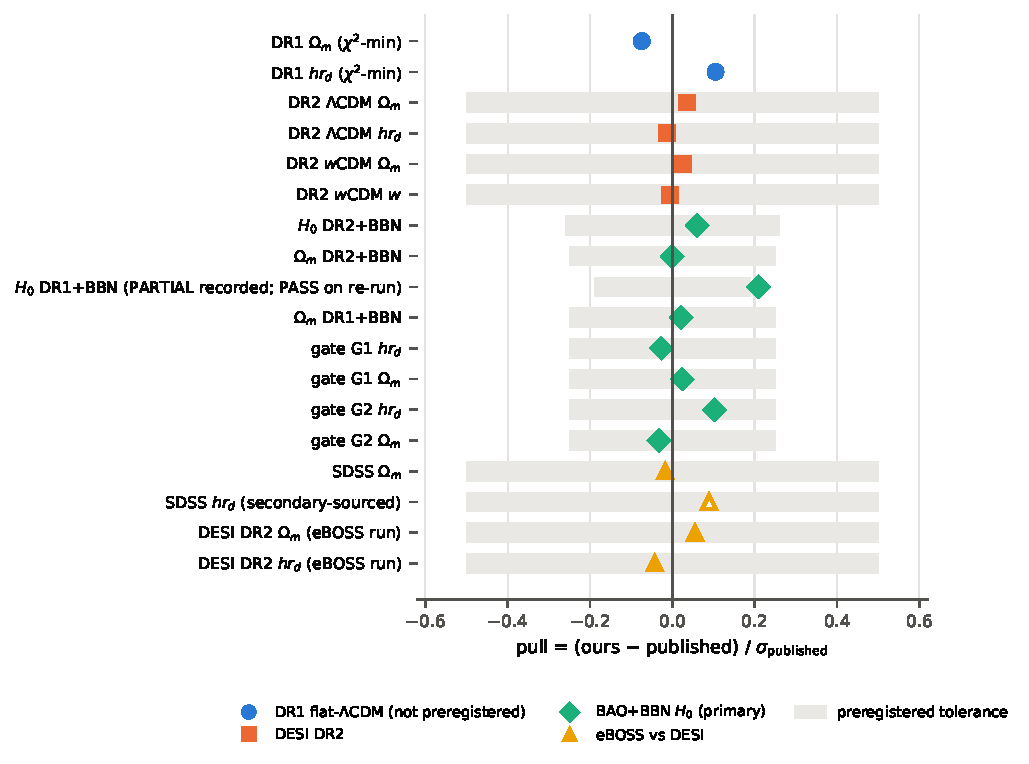
\includegraphics[width=0.92\textwidth]{fig_pulls.pdf}
\caption{Pulls of every numeric target, from the result JSONs by \texttt{make\_figures.py}. Grey bands show each target's preregistered
tolerance; they are tolerances, not error bars, and the pulls are not independent-sample significances (same data and priors on both sides). The DR1 run was not preregistered and has none. The hollow triangle (SDSS $hr_d$) marks a target taken from a secondary
source, which is excluded from the eBOSS tolerance rule. H0 secondary (fitting-formula) pulls are omitted here. They are listed in
Table~\ref{tab:h0} and shown in Fig.~\ref{fig:h0}.}\label{fig:pulls}
\end{figure}

\subsection{DESI DR1, flat $\Lambda$CDM}\label{sec:dr1}
Table~\ref{tab:dr1}. Two independently coded predictors agree exactly, and a brute-force $\rgNgrid\times\rgNgrid$ grid (steps $\rgStepOm$ in $\Omega_m$ and $\rgStepHrd$\,Mpc in $hr_d$) gives
$\Omega_m=\dOneGridOm$ and $hr_d=\dOneGridHrd$ ($\chi^2=\rgGridChi$), $\rgNodesOm$ and $\rgNodesHrd$ grid steps from the optimizer minimum along the degeneracy, i.e.\ within about one grid step. Table~\ref{tab:dr1} compares our $\chi^2$ minimum with DESI's posterior mean (eq.~4.1). The fetched DR1 paper also gives
the \emph{matched} target, its best-fit model: $\Omega_m=\rdPubOm$ and $H_0r_d=\rdPubHrd\times100$\,km\,s$^{-1}$ (Fig.~1 caption), with
$\chi^2=\rdPubChi$ for 10 degrees of freedom (Sec.~3.2)~\cite{desi2024vi}. Our $\Omega_m=\dOneOm$ and $hr_d=\dOneHrd$ agree with it to the printed
precision. Our $\chi^2_{\min}=\dOneChi$ for $\dOneDof$ degrees of freedom is higher by $\rdMzero$ on the same public data vector and covariance
(sha256 in Table~\ref{tab:data}). We tested background physics as the cause (\texttt{results/cosmo\_synthesis/dr1\_chi2\_offset\_check.py}): adding
radiation, or replacing the analytic distances by a CAMB background with massless neutrinos or with one $0.06$\,eV neutrino, changes $\chi^2_{\min}$ by at
most $\rdMaxChange$, leaving an offset of $\rdMthree$ in the DESI-like CAMB case. \textbf{The offset is unexplained}; it may come from a difference in the
likelihood inputs or the minimizer used by DESI, which we cannot inspect. The DR2 run later re-fitted DR1 with the posterior-mean estimator and obtained
$\Omega_m=\dTwoIOm$ (pull $\dTwoIOmP$) and $hr_d=\dTwoIHrd$ (pull $\dTwoIHrdP$).
\begin{table}[h]\centering\caption{DESI DR1 flat $\Lambda$CDM. Source: \dOneSource{} (eq.~4.1).}\label{tab:dr1}
\begin{tabular}{lccccc}
\toprule
Quantity & Ours ($\chi^2$-min) & $\sigma$ & Target & $\sigma_{\rm target}$ & Pull \\
\midrule
$\Omega_m$ & $\dOneOm$ & -- & $\dOneTOm$ & $\dOneTOmS$ & $\dOnePullOm$ \\
$h r_d$ [Mpc] & $\dOneHrd$ & -- & $\dOneTHrd$ & $\dOneTHrdS$ & $\dOnePullHrd$ \\
\bottomrule
\end{tabular}
\end{table}

\subsection{DESI DR2, $\Lambda$CDM and $w$CDM}
Table~\ref{tab:dr2}. Primary estimator: emcee posterior mean and standard deviation ($\dTwoNsteps$ steps per chain, converged under
the $50\tau$ rule). The largest emcee-minus-grid difference is $\dTwoEmceeGrid$ emcee $\sigma$. The correlation
$r(\Omega_m, hr_d)=\dTwoCorr$ compares with the published $\dTwoCorrT$, and the best-fit $\chi^2$ is $\dTwoChi$ for $\dTwoDof$ degrees of
freedom. The $w$CDM $hr_d=\dTwoWHrd\pm\dTwoWHrdS$\,Mpc is report-only, because no published value was found.
\begin{table}[h]\centering\small\caption{DESI DR2 BAO only (\texttt{results/desi\_dr2\_bao/fit.json}).}\label{tab:dr2}
\resizebox{\textwidth}{!}{\begin{tabular}{lcccccp{4.2cm}}
\toprule
Quantity & Ours & $\sigma$ & Target & $\sigma_{\rm t}$ & Pull & Source \\
\midrule
$\Lambda$CDM $\Omega_m$ & $\dTwoLOm$ & $\dTwoLOmS$ & $\dTwoLOmT$ & $\dTwoLOmTS$ & $\dTwoLOmP$ & \scriptsize arXiv:2503.14738v3 eq.(17) p.19 and Table V (DESI, LCDM); identical in v1 eq.(17) \\
$\Lambda$CDM $h r_d$ [Mpc] & $\dTwoLHrd$ & $\dTwoLHrdS$ & $\dTwoLHrdT$ & $\dTwoLHrdTS$ & $\dTwoLHrdP$ & \scriptsize arXiv:2503.14738v3 eq.(17) p.19; identical in v1 \\
$w$CDM $\Omega_m$ & $\dTwoWOm$ & $\dTwoWOmS$ & $\dTwoWOmT$ & $\dTwoWOmTS$ & $\dTwoWOmP$ & \scriptsize arXiv:2503.14738v3 Table V, wCDM row 'DESI' \\
$w$CDM $w$ & $\dTwoWw$ & $\dTwoWwS$ & $\dTwoWwT$ & $\dTwoWwTS$ & $\dTwoWwP$ & \scriptsize arXiv:2503.14738v3 Table V, wCDM row 'DESI' \\
\bottomrule
\end{tabular}
}\end{table}

\subsection{BAO+BBN inverse distance ladder}
Table~\ref{tab:h0}; sources in Table~\ref{tab:h0src}. The primary DR2 result passes every PASS condition. The DR1 check is
\hzPTwoV: $|\Delta H_0|=\hzPTwoD$ exceeds the strict window by $\hzTTwoMargin$\,\kms, which is comparable to our posterior-mean Monte
Carlo error of $\hzTTwoMC$. DESI's own posterior-mean sampling error is not published; its stated convergence floor (ESS $\gtrsim10^3$, \cite[Sec.~2.5]{desi2024vi})
implies up to about $\rtDesiMC$ on the quoted $\hzTTwo$, plus $\pm0.005$ rounding. The combined resolution is then about $\rtComb$, so the margin is $\rtMarginComb$ of it and
the strict/soft boundary is not statistically resolved (as the \texttt{T2\_boundary\_resolution} note in \texttt{fit.json} already states). The preregistered rule gives
PARTIAL for the recorded run, and PARTIAL is what that run reports; re-execution under a different numerical environment gives PASS (next paragraph), so we do
not present PARTIAL as a stable property of the analysis. A post-hoc diagnostic, which does
\emph{not} change the verdict: DR1 quotes $hr_d=\hzHrdQuoteEight$ in one section and $\hzHrdQuoteSix$ in another. Propagating these gives implied $H_0$
excesses of $\hzPostHocEight$ and $\hzPostHocSix$\,\kms{} ($\rtLo$--$\rtHi$ across the rounding of the first, $\pm\rtMCH$ from the G2 chain). The G2 gate used the first value. As shown in Sec.~\ref{sec:h0prot}, the gate tolerance itself admits
offsets of this size. \emph{Code deviation:} \texttt{scripts/bao\_bbn\_h0/fit\_real.py} (line 262) passes gate G1 into \texttt{verdict\_T2}, although the
preregistration defines gate G2 for the DR1 check. G2 \rgGTwoPassed{} (its \texttt{passed} field in \texttt{fit.json}), so the T2 verdict is unchanged;
the script is frozen and outside this synthesis' write scope.

\textbf{Numerical-environment dependence (found by the round-3 referee, confirmed here).}\label{sec:env}
The machine has two Python environments: \texttt{venv-pta} (Python \evPtaPy, numpy \evPtaNp, scipy \evPtaSp) and \texttt{venv-cosmo} (Python \evCosPy, numpy \evCosNp,
scipy \evCosSp), both with emcee \evEmcee. No run JSON records its interpreter. We re-ran the frozen \texttt{fit\_real.py} in isolated copies under both,
changing only the chain output directory (\texttt{results/cosmo\_synthesis/round3\_env\_rerun\_setup.py}, \texttt{round3\_response\_checks.py}; the two re-run outputs are kept as \texttt{round3\_rerun\_fit\_venv\_\{pta,cosmo\}.json}, hashes in Table~\ref{tab:sha}). Under
\texttt{venv-pta}, $\rePtaNdiff$ of $\rePtaNcomp$ numeric leaves of \texttt{fit.json} differ: the recorded H0 run was produced by \texttt{venv-pta}. Under
\texttt{venv-cosmo}, $\reCosNdiff$ of $\reCosNcomp$ differ. MAP $H_0$ values agree to $\reMapMax$, but the posterior means move by up to $\reShiftMC$ Monte Carlo
errors: primary T1 $H_0=\rePOneH$ (\rePOneV), \textbf{primary T2 $H_0=\rePTwoH$, $|\Delta H_0|=\rePTwoD$, i.e.\ \rePTwoV} instead of the recorded $\hzPTwoD$ (\hzPTwoV),
secondary T1 \reSOneV{} and secondary T2 $|\Delta H_0|=\reSTwoD$ (\reSTwoV). Gate G2's $hr_d$ mean becomes $\reGTwoHrd$\,Mpc; the implied $H_0$ shift, computed as in Sec.~\ref{sec:h0prot}, becomes $\reGTwoImpl$\,\kms, inside the range quoted there.
Integer leaves (chain lengths and burn-in) also differ, because the chains stop adaptively. The round-3 referee found the DR2 $\Lambda$CDM chain bit-identical under both interpreters; we did not repeat that check. The preregistration
names no interpreter, so both executions are equally valid applications of the preregistered rule. The primary T2 label is therefore \textbf{PARTIAL in the
recorded run and PASS on re-execution}; its margin over the strict window ($\hzTTwoMargin$) is about one Monte Carlo error, and chains of the recorded length cannot resolve
it. A preregistered verdict whose margin can be one MC error should either fix a chain long enough that the MC error is much smaller than the margin, or be stated
on a deterministic estimator (the MAP, or a posterior mean with a preregistered MC floor).

\textbf{Formula-versus-CAMB shift.} Exact CAMB versus the fitting formula moves the MAP $H_0$ by $\fsMapOne$ (DR2) and $\fsMapTwo$ (DR1), stable to $10^{-7}$
across both environments. The posterior-mean differences, $\hzPmSOne\pm\fsMcOne$ (DR2) and $\hzPmSTwo\pm\fsMcTwo$ (DR1) in the recorded run and $\fsCosOne$ / $\fsCosTwo$
under \texttt{venv-cosmo}, are dominated by Monte Carlo noise; the smaller DR1 value is not a smaller systematic. The largest fitting-formula error measured against CAMB is $\hzAubCambMaxPct$\,\%.
Aubourg et al.\ state 0.021\% accuracy for $N_{\rm eff}=3.046$ and parameters within $3\sigma$ of Planck~\cite{aubourg2015}; $\raNexceed$ of our
$\raNpts$ validation points exceed that figure, including the largest one at $(\omega_b,\omega_{\rm cdm})=(\raWorstOb,\raWorstOc)$, which lies inside
the proxy validity window used in the preregistration. Our CAMB table uses $N_{\rm eff}=3.044$, whereas Aubourg's statement assumes 3.046. Re-running CAMB (v\raCambVer)
at $N_{\rm eff}=3.046$ for the same points (\texttt{round2\_response\_checks.json}, key \texttt{aubourg\_neff}) shows that $r_d$ at 3.044 exceeds $r_d$ at 3.046 by
$(\raShiftLo$--$\raShiftHi)\times10^{-5}$, close to the $\raEqSeventeen\times10^{-5}$ of Aubourg's eq.~(17) factor. Against the 3.046 CAMB values, $\raNexceedSix$ of the $\raNpts$ points
still exceeds 0.021\% (largest $\raMaxSixPct$\,\%). Part of the remainder is a convention in the validation code (found by the round-3 referee):
\texttt{rd\_camb\_table.py} compares CAMB and eq.~(16) at equal $\Omega_m h^2$, which is what the fit samples, and so evaluates eq.~(16) at
$\omega_{cb}=\omega_b+\omega_{\rm cdm}+(\omega_\nu^{\rm CAMB}-\omega_\nu^{\rm Aubourg})$, i.e.\ $\aoOffset$ above the CAMB grid point's $\omega_b+\omega_{\rm cdm}$.
Aubourg's accuracy statement is at given $\omega_{cb}$. Evaluated at the grid point's own $\omega_b+\omega_{\rm cdm}$, the largest deviation from the $N_{\rm eff}=3.046$
CAMB values is $\aoMatchedPct$\,\% ($\aoNexceed$ point above 0.021\%; \texttt{round3\_response\_checks.json}, key \texttt{aubourg\_omega\_cb}). The $N_{\rm eff}$ convention
and this $\omega_{cb}$ convention together explain most of the excess; the residual of order $10^{-5}$ was not traced further. The preregistered comparison (against the 3.044 table) is the one reported above.
The CAMB anchor at the Planck 2018 best fit gives $r_{\rm drag}=\hzCambAnchor$\,Mpc; the preregistration cites $\hzCambAnchorPre$.
\begin{table}[h]\centering\small\caption{BAO+BBN $H_0$ (\texttt{results/bao\_bbn\_h0/fit.json}, key \texttt{pulls}; recorded run, \texttt{venv-pta}). Values in \kms{} for $H_0$
and Mpc for $hr_d$. ``secondary'' is the preregistered fitting-formula analysis and is identical to the hash-locked first attempt in the same numerical environment. The
``shared'' gate rows are BAO-only reproductions. $^\ddagger$Environment-dependent: re-executing the frozen script under \texttt{venv-cosmo} gives $|\Delta H_0|=\rePTwoD$
(strict rule met); the boundary is within Monte Carlo resolution (Sec.~\ref{sec:env}).}\label{tab:h0}
\resizebox{\textwidth}{!}{\begin{tabular}{llcccccl}
\toprule
Analysis & Target & Ours & $\sigma$ & Target & $\sigma_{\rm t}$ & Pull & Strict rule met \\
\midrule
primary & T1\_H0 & $\hzRowav$ & $\hzRowas$ & $\hzRowat$ & $\hzRowats$ & $\hzRowap$ & yes \\
primary & T1b\_Omega\_m & $\hzRowbv$ & $\hzRowbs$ & $\hzRowbt$ & $\hzRowbts$ & $\hzRowbp$ & yes \\
primary & T2\_H0 & $\hzRowcv$ & $\hzRowcs$ & $\hzRowct$ & $\hzRowcts$ & $\hzRowcp$ & no (soft: yes) [re-run: yes]$^\ddagger$ \\
primary & T2b\_Omega\_m & $\hzRowdv$ & $\hzRowds$ & $\hzRowdt$ & $\hzRowdts$ & $\hzRowdp$ & yes \\
secondary & T1\_H0 & $\hzRowev$ & $\hzRowes$ & $\hzRowet$ & $\hzRowets$ & $\hzRowep$ & yes \\
secondary & T1b\_Omega\_m & $\hzRowfv$ & $\hzRowfs$ & $\hzRowft$ & $\hzRowfts$ & $\hzRowfp$ & yes \\
secondary & T2\_H0 & $\hzRowgv$ & $\hzRowgs$ & $\hzRowgt$ & $\hzRowgts$ & $\hzRowgp$ & no (soft: yes) \\
secondary & T2b\_Omega\_m & $\hzRowhv$ & $\hzRowhs$ & $\hzRowht$ & $\hzRowhts$ & $\hzRowhp$ & yes \\
shared & G1\_hrd & $\hzRowiv$ & $\hzRowis$ & $\hzRowit$ & $\hzRowits$ & $\hzRowip$ & yes \\
shared & G1\_Omega\_m & $\hzRowjv$ & $\hzRowjs$ & $\hzRowjt$ & $\hzRowjts$ & $\hzRowjp$ & yes \\
shared & G2\_hrd & $\hzRowkv$ & $\hzRowks$ & $\hzRowkt$ & $\hzRowkts$ & $\hzRowkp$ & yes \\
shared & G2\_Omega\_m & $\hzRowlv$ & $\hzRowls$ & $\hzRowlt$ & $\hzRowlts$ & $\hzRowlp$ & yes \\
\bottomrule
\end{tabular}
}\end{table}
\begin{table}[h]\centering\caption{H0 target sources, read from \texttt{preregistration.json} (not editable after the fit). For G2 the string names the DR1 abstract,
but the fetched abstract quotes only $\Omega_m$ and $H_0$; $r_dh=101.8\pm1.3$ is in eq.~(4.1) and Sec.~8 of~\cite{desi2024vi}.}\label{tab:h0src}
\resizebox{\textwidth}{!}{\begin{tabular}{lp{11cm}}
\toprule
Target & Source (preregistration) \\
\midrule
T1 & \scriptsize arXiv:2503.14738 eq. (19) and Table V row DESI+BBN (no CMB theta*) \\
T1b & \scriptsize arXiv:2503.14738 Table V \\
T2 & \scriptsize arXiv:2404.03002 eq. (4.4), Table 3 (no CMB theta*) \\
T2b & \scriptsize arXiv:2404.03002 Table 3 \\
G1 & \scriptsize arXiv:2503.14738 eq. (17) \\
G2 & \scriptsize arXiv:2404.03002 abstract/Sec. 8 \\
\bottomrule
\end{tabular}
}\end{table}

\begin{figure}[h]\centering
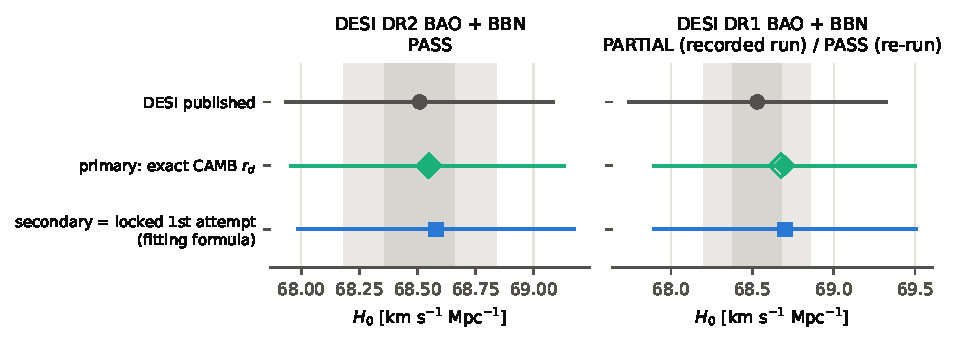
\includegraphics[width=0.95\textwidth]{fig_h0.pdf}
\caption{$H_0$ from BAO+BBN. The primary analysis uses the exact CAMB $r_d$ (amendment~1). The secondary analysis uses the preregistered
fitting formula and, in the recorded environment, equals the hash-locked, unread first attempt. Filled symbols: recorded run (\texttt{venv-pta}); hollow diamond: the primary posterior mean
when the same frozen script is re-executed under \texttt{venv-cosmo} (Sec.~\ref{sec:env}). The dark band is the strict window ($\pm\hzStrict$) and the light band
the soft window ($\pm\hzSoft$) around the DESI value.}\label{fig:h0}
\end{figure}

\subsection{SDSS/eBOSS versus DESI DR2}
Table~\ref{tab:eboss}. The SDSS $(\Omega_m, hr_d)$ correlation we find is $\ebSCorr$; SDSS does not publish it. The baseline and
Gaussian-summary SDSS likelihoods differ by $\ebBaseVsGauss\sigma$ in $\Omega_m$. The DESI numbers here come from an independent re-fit
with shorter chains, so they differ slightly from Table~\ref{tab:dr2}.
\begin{table}[h]\centering\small\caption{eBOSS vs DESI (\texttt{results/eboss\_vs\_desi/fit.json}). $^\dagger$Taken from a secondary source
(DR1 quoting SDSS). We did not find it in the fetched pages of the primary paper, so it is not counted toward the tolerance rule.}\label{tab:eboss}
\resizebox{\textwidth}{!}{\begin{tabular}{lcccccp{4.3cm}}
\toprule
Quantity & Ours & $\sigma$ & Target & $\sigma_{\rm t}$ & Pull & Source \\
\midrule
SDSS $\Omega_m$ & $\ebSOm$ & $\ebSOmS$ & $\ebSOmT$ & $\ebSOmTS$ & $\ebSOmP$ & \scriptsize arXiv:2007.08991 Table IV (BAO, flat LCDM): Omega\_DE = 0.701 +0.017/-0.015 -> Om = 1-Omega\_DE = 0.299 +0.015/-0.017; symmetric 0.016 also quoted by arXiv:2404.03002 Sec. 4.1 \\
SDSS $h r_d$ [Mpc]$^\dagger$ & $\ebSHrd$ & $\ebSHrdS$ & $\ebSHrdT$ & $\ebSHrdTS$ & $\ebSHrdP$ & \scriptsize arXiv:2404.03002 Sec. 4.1 citing [139]=arXiv:2007.08991 \\
DESI DR2 $\Omega_m$ & $\ebDOm$ & $\ebDOmS$ & $\ebDOmT$ & $\ebDOmTS$ & $\ebDOmP$ & \scriptsize arXiv:2503.14738 eq. (17) \\
DESI DR2 $h r_d$ [Mpc] & $\ebDHrd$ & $\ebDHrdS$ & $\ebDHrdT$ & $\ebDHrdTS$ & $\ebDHrdP$ & \scriptsize arXiv:2503.14738 eq. (17); corr r = -0.92 \\
\bottomrule
\end{tabular}
}\end{table}

\subsection{Derived quantities not quoted in the fetched DESI text}
Table~\ref{tab:derived}. DR2 does test consistency with DR1 and with SDSS, but at the level of distances. It compares DR1 and DR2
bin by bin with a correlated joint uncertainty and a KS test, and compares SDSS with DESI per redshift bin in $\alpha_{\rm iso}$ and
$\alpha_{\rm AP}$~\cite[Sec.~III.C]{desi2025dr2}. In the fetched text we found no parameter-level $(\Omega_m, hr_d)$ number for
either comparison. The quantities below complement those checks and do not replace them.

(a) DR1 and DR2 share data. We use the nested uncertainty on their difference,
$\sigma_{\rm nested}^2=\sigma_{\rm DR1}^2-\sigma_{\rm DR2}^2$, which gives $\shRatioOwn\sigma_{\rm nested}$. DR2 describes its own DR1--DR2 comparison as
assuming perfect correlation, but computes $\sigma^2=\sigma_{\rm DR2}^2+\sigma_{\rm DR1}^2-2C\sigma_{\rm DR1}\sigma_{\rm DR2}$ with $C=\sqrt{N_{\rm DR1}/N_{\rm DR2}}$
per galaxy/quasar tracer ($C=0.61$ for Ly$\alpha$)~\cite[Sec.~III.C.1 and footnote~12]{desi2025dr2}; with $\sigma\propto N^{-1/2}$ this is the nested form for the galaxy and quasar bins, which is all the parameter-level argument needs. Taking $C=1$ literally at the
parameter level gives $\sigma=|\sigma_{\rm DR1}-\sigma_{\rm DR2}|=\rcSigCone$ and $\rcRatioCone\sigma$, and the independent convention gives $\shRatioInd\sigma$.
The $\sigma\propto N^{-1/2}$ step is only approximate: Kim, Mota \& Tamosiunas~\cite{kim2026}, who model the DR1-inside-DR2 nesting explicitly with a
year-scaling decomposition (their Appendix~B.2), report that the published per-bin covariances ``straddle'' the ratio $C_{\rm DR2}=C_{\rm DR1}/3$ that pure year scaling
implies, at 0.22--0.49 (median 0.32). Our $\sigma_{\rm nested}$ is therefore an approximation, bracketed by the $C=1$ and independent conventions.
All three conventions agree that the shift is insignificant. The published means imply $\Delta\Omega_m=\shPub$.

(b) The SDSS--DESI DR2 tension applies DESI's parameter-difference statistic (eq.~18 of~\cite{desi2025dr2}) to BAO-only $(\Omega_m, hr_d)$ under the
independent-survey assumption. DR2 states that the two surveys are consistent but gives no number for this pair of parameters. For DR1, the DESI
paper gives a qualitative parameter-level statement: ``no significant difference in $\Omega_m$ and a shift of just $\sim1\sigma$ in $r_dh$''~\cite[Sec.~3.3]{desi2024vi}.
Two other papers compare SDSS and DESI and reach different-sounding conclusions because they ask different questions. Ghosh \&
Bengaly~\cite{ghosh2024} reconstruct $H(z)$ and $q(z)$ non-parametrically (Gaussian processes) from $D_H/r_d$ alone, for DESI DR1, with a Planck
$r_d$, and find the reconstructions ``significantly inconsistent''; this is not a parameter-level test in $(\Omega_m, hr_d)$. Ferri, Ruchika \&
Melchiorri~\cite{ferri2026} compare SDSS DR16 and DESI DR2 combined with Planck in the CPL model and find offsets in $w_0$ and $q_0$ of about
$1.1\sigma$. Our number is narrower: BAO alone, flat $\Lambda$CDM, $(\Omega_m, hr_d)$, eq.~(18). Before any fit, the preregistration had bounded $N_\sigma$ to
$\ebLitLo$--$\ebLitHi$ from published means alone, so the value is an application of a known statistic, not a surprise. The 1D
differences are $\ebOneDOm\sigma$ ($\Omega_m$) and $\ebOneDHrd\sigma$ ($hr_d$). Because the surveys overlap, the independent-survey $N_\sigma$ is a lower
bound only under the assumption that the cross-covariance is positive; with $X+X^{\rm T}$, $X=\rho\sqrt{C_S}\sqrt{C_D}$, subtracted from $C_S+C_D$ (the covariance of a
difference), $N_\sigma$ rises to
$\roNsigFiftySeven$ at $\rho=0.57$ (PTE $\roPTEFiftySeven$). The value $0.57$ is DR2's estimate for one bin pair (LRG2 and eBOSS LRG), the only pair for which DR2 quotes $C$~\cite[Sec.~III.C.2]{desi2025dr2};
applying it to the whole parameter-level covariance is an illustration, not an estimate. DR2 uses the same lower-bound logic for its own distance-level comparison:
for that bin pair the discrepancy is $\sim2.6\sigma$ with $C\approx0.57$, and ``although the assumption of no correlation is less plausible, it sets a lower limit of the
discrepancy at the $1.9\sigma$ level''~\cite[Sec.~III.C.2]{desi2025dr2} ($2.3\sigma$ and $1.5\sigma$ with DESI's reanalysis of SDSS; our eBOSS run uses the
published SDSS DR16 likelihoods, to which the $1.9$--$2.6\sigma$ figures refer). Our parameter-level $N_\sigma=\ebNsig$ therefore does not mean that there is no tension anywhere: the
LRG2/eBOSS-LRG bin pair (the one DR1 had flagged at $\sim3\sigma$) is at $1.9$--$2.6\sigma$ by DR2's own numbers, and the two-parameter BAO-only fit averages over bins.

(c) The CAMB-versus-formula $H_0$ shift, measured deterministically between MAP points as $\fsMapOne$ (DR2) and $\fsMapTwo$\,\kms{} (DR1), equals the
propagation of the \emph{measured} formula error near the posterior ($-\fpEpsPct$\,\% at the first validation point, which gives $\fpPredOne$ and $\fpPredTwo$ through
$\Delta\ln h=-\epsilon/(d\ln hr_d/d\ln h)$ with the slopes of \texttt{fixround\_diagnostics.json}). Aubourg et al.'s stated 0.021\% would give only about $\fpStatedOne$.
The shift therefore does not confirm the stated accuracy figure; it is consistent with the exceedances of 0.021\% reported in Sec.~\ref{sec:env}, and it is not a new quantity.
\begin{table}[h]\centering\small\caption{Derived quantities.}\label{tab:derived}
\resizebox{\textwidth}{!}{\begin{tabular}{p{6.3cm}cp{8.8cm}}
\toprule
Quantity & Value & Definition / source key \\
\midrule
DR1$\to$DR2 shift $\Delta\Omega_m$ (DR2 run, emcee means) & $\shDelta$ & \scriptsize \texttt{DR1\_to\_DR2\_shift.Delta\_Om} \\
$\Delta\Omega_m/\sigma_{\rm nested}$ (own $\sigma_{\rm nested}=\shSigNestOwn$) & $\shRatioOwn$ & \scriptsize $\sigma_{\rm nested}^2=\sigma_{\rm DR1}^2-\sigma_{\rm DR2}^2$; \texttt{Delta\_over\_sigma\_nested\_own} \\
$\Delta\Omega_m/\sigma_{\rm nested}$ (preregistered $\sigma=\shSigNestPre$) & $\shRatioPre$ & \scriptsize \texttt{Delta\_over\_sigma\_nested\_prereg} \\
$\Delta\Omega_m/\sigma_{\rm indep}$ (wrong if nested; for comparison) & $\shRatioInd$ & \scriptsize \texttt{Delta\_over\_sigma\_independent\_own} \\
$\Delta\Omega_m/|\sigma_{\rm DR1}-\sigma_{\rm DR2}|$ ($C=1$ bracket) & $\rcRatioCone$ & \scriptsize \texttt{round1\_response\_checks.json: dr1\_dr2\_conventions.ratio\_C1} \\
SDSS--DESI DR2 tension, $(\Omega_m, h r_d)$, 2 dof & $N_\sigma=\ebNsig$ & \scriptsize $\chi^2=\ebChi$, PTE $=\ebPTE$; \texttt{tension.primary\_emcee\_moments} \\
\quad same, grid / MAP+Laplace / KDE shift & $\ebNsigGrid$ / $\ebNsigMAP$ / $\ebNsigKDE$ & \scriptsize \texttt{tension.\{grid\_moments, MAP\_laplace, posterior\_parameter\_shift\_KDE\}} \\
\quad same, with $X+X^{\rm T}$, $X=\rho\sqrt{C_S}\sqrt{C_D}$, subtracted, $\rho=0.57$ (illustration) & $N_\sigma=\roNsigFiftySeven$ & \scriptsize \texttt{round1\_response\_checks.json: overlap\_sensitivity} \\
$H_0$ shift, exact CAMB $r_d$ minus fitting formula, DR2, MAP (deterministic; equals the propagated measured formula error, which exceeds Aubourg's stated 0.021\%; not new) & $\fsMapOne$ km/s/Mpc & \scriptsize \texttt{round3\_response\_checks.json}, key \texttt{formula\_shift}, \texttt{map\_diff} \\
\quad same, DR1, MAP & $\fsMapTwo$ km/s/Mpc & \scriptsize \texttt{...T2\_DR1.map\_diff} \\
\quad posterior-mean differences DR2 / DR1 (MC-noise dominated) & $\hzPmSOne\pm\fsMcOne$ / $\hzPmSTwo\pm\fsMcTwo$ & \scriptsize \texttt{measured\_formula\_systematic}; MC error from chain std/$\sqrt{\rm ESS}$ \\
Wrong neutrino bookkeeping (N4), $\Delta H_0$ (MAP) & $\hzNfourD$ km/s/Mpc & \scriptsize $\Delta\chi^2=\hzNfourChi$; \texttt{controls/N4.json} \\
\bottomrule
\end{tabular}
}\end{table}

\begin{table}[h]\centering\small\caption{Dual-environment Lean check (\texttt{results/cosmo\_synthesis/lean\_dual\_check.json}, revision~2 of the checker). ``\#print axioms'' counts
commands in comment-stripped source. Wall times are single measurements on a shared machine.}\label{tab:lean}
\resizebox{\textwidth}{!}{\begin{tabular}{lcccccc}
\toprule
File & Theorems & \#print axioms & Env 1 rc & Env 1 time [s] & Env 2 rc & Env 2 time [s] \\
\midrule
\texttt{BAO\_FlatLCDM.lean} & $\lnAN$ & $\lnAPA$ & $\lnARcOne$ & $\lnATOne$ & $\lnARcTwo$ & $\lnATTwo$ \\
\texttt{DESI\_DR2\_wCDM.lean} & $\lnBN$ & $\lnBPA$ & $\lnBRcOne$ & $\lnBTOne$ & $\lnBRcTwo$ (BLOCKED\_ENV) & $\lnBTTwo$ \\
\texttt{BAO\_BBN\_H0.lean} & $\lnCN$ & $\lnCPA$ & $\lnCRcOne$ & $\lnCTOne$ & $\lnCRcTwo$ & $\lnCTTwo$ \\
\texttt{BAO\_Consistency.lean} & $\lnDN$ & $\lnDPA$ & $\lnDRcOne$ & $\lnDTOne$ & $\lnDRcTwo$ & $\lnDTTwo$ \\
\bottomrule
\end{tabular}
}\end{table}
\begin{table}[h]\centering\small\caption{Elenchus ledgers. ``A audited (model)'' counts Tier~A rows whose audit is a non-empty object naming an auditor (all are model referees).
``Audit hash = current file'' counts those audits whose recorded source sha256 equals the current Lean file. rc is the
gate exit code (DR1: from the DR2 run's parent-ledger control). Tier~B here means a seeded floating-point harness on sha256-verified inputs; Elenchus's own Tier~B is exact
$\mathbb{Q}/\mathbb{Z}$ arithmetic and would file these rows at X (Sec.~\ref{sec:ledger}).}\label{tab:ledger}
\resizebox{\textwidth}{!}{\begin{tabular}{lcccccccc}
\toprule
Run & Claims & A & B & L & C & A audited (model) & audit hash = current file & gate rc \\
\midrule
DR1 flat-$\Lambda$CDM & $\lAN$ & $\lATA$ & $\lATB$ & $\lATL$ & $\lATC$ & $\lAAud/\lATA$ & $\lABound/\lAAud$ & $\lARc$ \\
DESI DR2 & $\lBN$ & $\lBTA$ & $\lBTB$ & $\lBTL$ & $\lBTC$ & $\lBAud/\lBTA$ & $\lBBound/\lBAud$ & $\lBRc$ \\
BAO+BBN $H_0$ & $\lCN$ & $\lCTA$ & $\lCTB$ & $\lCTL$ & $\lCTC$ & $\lCAud/\lCTA$ & $\lCBound/\lCAud$ & $\lCRc$ \\
eBOSS vs DESI & $\lDN$ & $\lDTA$ & $\lDTB$ & $\lDTL$ & $\lDTC$ & $\lDAud/\lDTA$ & $\lDBound/\lDAud$ & $\lDRc$ \\
\bottomrule
\end{tabular}
}\end{table}

\section{What is and is not new}\label{sec:new}
\textbf{Not new.} Every cosmological parameter here reproduces a published value from the same public likelihood files, using methods
the DESI and SDSS papers describe. Nothing here is a new measurement or a new constraint.

\textbf{Prior work we found.} The first draft's search used four alphaXiv queries (LLM agents reproducing cosmology analyses; formal verification of
physics in Lean or other proof assistants; HepLean/PhysLean; benchmarks of agents reproducing astrophysics papers); their exact strings and dates
were not recorded. For this revision we ran two further queries, on SDSS--DESI consistency and on blind analysis and preregistration for agents,
and recorded them exactly (\texttt{literature\_search\_log\_round1.json} in \texttt{results/cosmo\_synthesis/}). Those queries missed two axes, pre-run cryptographic
commitment of cosmological analyses and autonomous analysis agents with model review and an unblinding gate. The round-2 novelty referee supplied the papers below
by arXiv id; we fetched and read each before citing it (\texttt{literature\_search\_log\_round2.json}). None of these searches covered agent-executed reproduction
outside cosmology and HEP; the round-3 novelty referee's sweep without the word ``BAO'' found three such pipelines on its first page. For this revision we ran one
recorded sweep on that axis and read those three papers and three further ones by arXiv id (\texttt{literature\_search\_log\_round3.json}). Only papers we read are cited.

For agent-executed reproduction of a published result against numeric targets, the most direct precedent is SHARP~\cite{sharp2026}: a Claude Code
pipeline (claude-opus-4.6) whose initiating prompt names the paper and the target metrics, with Paper Analyst, Code, Test, Statistician and Critic subagents and human
review at checkpoints; it reports three independent runs against the published ParticleNet-Lite numbers, validates checkpoints with an external evaluation script written by
a human expert, and records a truth-label-leakage failure that ``went undetected by automated tests'', the class of problem our N4 control targets. At scale,
Huang~\cite{huang2026scrutiny} runs a fresh Claude Code/Opus~4.6 agent on each of 111 open-access Quantum ESPRESSO papers, with a four-tier verdict (T1--T4) and a 12-paper
two-machine cross-check with no shared state, and matches 75.8\% of 571 claims within 5\% of the published value. A companion pipeline~\cite{huang2026grounded} reproduces
$k=5$ published anchors before any new computation and uses fresh-context adversarial review ``prompted to find rather than confirm''; its no-pilot ablation had the anchor
value in its own files yet never wrote the comparison, the failure mode that preregistered targets and tolerances address, and its note added reports that the anchor value itself
was not converged, so that single-anchor calibration gives ``consistency with published literature, not truth''. Our targets (DESI posterior means, and our unexplained DR1
$\chi^2$ offset) sit in the same epistemic position. For cosmology, the most direct precedent is cmbagent. Its 2024 workshop version~\cite{laverick2024} reproduced the published ACT DR6 lensing constraints with a human
approving each step, and its authors note that such output cannot be confirmed without redoing the analysis independently. Its Planning \& Control
mode~\cite{xu2025pc} runs ``with no human-in-the-loop at any point'' and serves as the analysis backend of Denario~\cite{denario2025}, an end-to-end
research-assistant system. Related systems
include agent-driven inference pipelines in which human redirection was decisive~\cite{borrett2026} (a competition entry, not a reproduction of a
published result), agentic cosmology frameworks and their caveats~\cite{xu2026}, and DarkAgents~\cite{darkagents2026}, which audits assumptions and
compares its results against a human analysis. The AI Cosmologist~\cite{moss2025} is an autonomous agentic system for cosmological and astronomical data analysis,
demonstrated on machine-learning tasks (Galaxy Zoo~2, Quijote) rather than on reproductions of published parameter constraints. Gandhi, Bolliet \& Zubeldia~\cite{gandhi2025}
extend cmbagent with plots treated as checkpoints that a vision-language model judges against generated rubrics, which also leaves auditable reasoning traces.
The nearest precedents for a model referee are cosmology-native: Denario's Review module writes a referee report (\texttt{referee.md})~\cite[Sec.~3.7]{denario2025},
and the VLM judge of~\cite{gandhi2025}; the AI Scientist~\cite{aiscientist} also uses an automated reviewer.
The closest architectural precedent for our design is JFC (``Just Furnish Context'', Moreno et al.~\cite{moreno2026}): a Claude Code orchestrator delegates to executor
and reviewer subagents, ``multi-agent review replaces the human feedback loop'', ``human oversight is concentrated at a single formal unblinding gate'', an append-only
experiment log records every phase transition, and one of its analyses is checked against, and consistent with, a published CMS $H\to\tau\tau$ measurement. In the pages of JFC and cmbagent that we
read we did not find preregistered numeric targets or hash-locked results; we do not claim that they lack them. SHARP's prompt does fix numeric targets, without
tolerances, controls or a lock; that, rather than the targets themselves, is what differs here.
Benchmark results on reproduction are mixed. Benchmarks built from whole papers report low scores: ReplicationBench~\cite{replicationbench} reports that the best model, Claude 4.5 Sonnet,
scores 22\% (Sec.~5.1 and Table~2; its abstract says ``under 20\%''), and PRBench~\cite{prbench} reports a best overall score of 34\%, a zero end-to-end
success rate, and fabricated outputs. Pipelines working from public inputs with a stated method report high agreement (SHARP; 75.8\% within 5\% in~\cite{huang2026scrutiny}),
as do our four runs, which start from public summary likelihoods with a published estimator. Collider-Bench~\cite{colliderbench} has agents reproduce LHC analyses and uses an LLM provenance judge that flags
FABRICATED runs whose values cannot be traced to an executed pipeline; this is the closest analogue of our re-running referee plus content-addressed evidence.
On the formal side, HepLean (now Physlib)~\cite{heplean,toobysmith2026} formalizes high-energy physics in Lean~4, a Lean formalization found a genuine
error in a widely cited 2HDM stability theorem~\cite{toobysmith2026}, and FormalScience~\cite{formalscience} autoformalizes physics in Lean with agents and
gives a taxonomy of semantic drift (e.g.\ ``abstraction elevation''), the class of problem behind our DR2 $z>-1\to z\ge0$ drift.

\textbf{Blind analysis.} The field's established safeguard against confirmation bias is blinding. Both target analyses were blind: DESI DR1 blinded
catalogs (redshift shifts for galaxies and quasars, an additive BAO-peak shift for Ly$\alpha$) until a prescribed set of validation tests
passed~\cite[Sec.~2.3.1]{desi2024vi}, with the scheme validated by Andrade et al.~\cite{andrade2024}, and DR2 applied ``strict catalog-level blinding'' with
pre-specified unblinding criteria~\cite[Secs.~II.A.1 and IX]{desi2025dr2}. Grosso, Mikuni \& Heinrich~\cite{grosso2026} recommend a blind-analysis-like
separation for agentic systems (optimize on simulation, reserve observed data for the final test) and note that ``No analogous verification infrastructure
exists for physics analyses'' to the role Lean plays for mathematics. Our setup is \emph{weaker} than a blind analysis: the targets were published and
visible to the agents, and the preregistrations were committed to git only after the fits. Preregistration and the hash-locked unread fit guard the
decision rules, not the agents' knowledge of the answer. It is also weaker than JFC~\cite{moreno2026} in this respect: JFC blinds its agents in stages (Asimov data,
then a 10\% subsample, then the full data) and requires a human to approve unblinding, whereas our pipeline has no blinding and no human gate at any point.
The published cosmology instance of our hash-lock safeguard is TOPO~\cite{topo2024}: the analyst signs an Analysis-Hash of code commits and input files and publishes it on
a timestamped medium (their example uses a public blockchain) before running, then publishes Merkle-tree roots over the time-ordered MCMC chain, so that a verifier can
re-run part of the chain and check it; it is demonstrated with Cobaya and CLASS on BAO likelihoods that include SDSS DR16. Our hash-locked unread fit and sha256
evidence blobs are a one-file instance of that idea, timestamped only by file mtime, and TOPO's timestamped commitment is exactly what our preregistrations lack.

\textbf{What is new, within the limits of that search.}
\begin{enumerate}
\item \emph{The combination of safeguards} applied to agent-executed cosmology:
  \begin{itemize}
  \item preregistered targets and tolerances;
  \item an amendment that hash-locks an unread earlier result and reports both analyses (a local version, timestamped only by file mtime, of the commitment that TOPO~\cite{topo2024} timestamps publicly);
  \item a subtle-bug control that the likelihood cannot detect;
  \item in-file, axiom-audited Lean statements of the model skeleton, checked in two environments (same toolchain) with \texttt{sorry} and axiom-smuggling controls;
  \item a tier-capped claim ledger with mutation controls;
  \item a re-running adversarial referee;
  \item a second-language port.
  \end{itemize}
  Each item exists elsewhere, the closest combined precedents being JFC~\cite{moreno2026} and, for reproduction against numeric targets, SHARP~\cite{sharp2026}, and our combination is weaker than the blind analyses of the target papers and than
  JFC's staged blinding and human gate in one respect (the answer was visible, and no person approved anything).
  We did not find these items combined in the literature we searched, and we do not claim priority beyond that.
\item \emph{Two derived consistency numbers} not quoted in the fetched text of~\cite{desi2025dr2,desi2024vi}: the DR1$\to$DR2 shift in
nested $\sigma$, and the BAO-only $(\Omega_m, hr_d)$ SDSS--DESI DR2 $N_\sigma$ from eq.~(18). Each is a simple function of public inputs.
\item \emph{Verification artifacts and an audit of the process}, including where it failed: a model audit clears the ledger gate, and the gate does
not check claim-to-evidence correspondence; the project's Lean runner could not gate worktree files; preregistration files were untracked; one
negative control was vacuous; one Lean statement drifted ($z>-1\to z\ge0$) and stays drifted in the shipped file for audit binding, although the preregistered domain
was shown to prove with the same tactics for the two positivity theorems; the eBOSS preregistered module
\texttt{BAO\_TensionStatistic.lean} (diagonal $\chi^2$) shipped as \texttt{BAO\_Consistency.lean} (full $2\times2$ covariance), a deviation disclosed in
the eBOSS README and paper; the H0 script passes gate G1 where the preregistration names G2; the H0 statement audits are bound to a stale source hash;
the first dual-check record was hand-corrected; the primary H0 DR1 verdict flips from PARTIAL to PASS when the frozen script is re-run under the project's other
Python environment, and no run recorded its interpreter; the ledgers' Tier~B is a local redefinition of Elenchus's exact-arithmetic tier; and defects were found in a
Rust reimplementation of CVODE.
\end{enumerate}

\section{Limitations}\label{sec:limits}
\begin{itemize}
\item \textbf{Partial result, environment-dependent.} The primary H0 DR1 check is PARTIAL ($|\Delta H_0|=\hzPTwoD$) in the recorded run (\texttt{venv-pta}) and PASS
($\rePTwoD$) when the same frozen script is re-executed under \texttt{venv-cosmo}; the two differ by $\reShiftMC$ Monte Carlo errors, so the strict boundary is not resolved and
neither label is a stable property of the analysis. The secondary DR1 check is PARTIAL in both. The gate-tolerance mechanism is consistent with the recorded PARTIAL but does not establish it: depending on which DR1 $hr_d$
is the reference and on its rounding, the mechanism accounts for $\rtMin$--$\rtMax$\,\kms{} ($\pm\rtMCH$) of the observed $\hzPTwoD$, and the explanation is post-hoc. The SDSS $hr_d$ target comes
from a secondary source.
\item \textbf{Incoherent H0 tolerances.} The preregistered gate tolerance ($0.25\sigma$ on $hr_d$) admits $H_0$ offsets of up to $\rgGOneMax$ / $\rgGTwoMax$\,\kms{},
beyond the strict window, so PASS versus PARTIAL does not isolate the BBN/$r_d$ step. A published BBN reaction-network systematic of up to $\sim0.5\sigma$ in $h$~\cite{akharman2026}
is also larger than the strict window. No tolerance was changed after the fits. The H0 script uses gate G1
in the T2 verdict where the preregistration names G2 (G2 passed; the verdict is unchanged; the frozen script was not edited).
\item \textbf{DR1 $\chi^2$ offset.} Our DR1 $\chi^2_{\min}$ exceeds DESI's by $\rdMzero$ on the same data; radiation and neutrino background choices do
not explain it. It remains open.
\item \textbf{Tier~A is model-audited, by the same model family.} Every statement audit was done by a Claude model reviewing Claude-written work, so producer and
verifier are not independent in vendor or training lineage, and automated review is reviewer-family dependent~\cite{ravideshik2026}. Two H0 theorems are unaudited. No person has checked
that any Lean statement means what its gloss claims. The Lean theorems are elementary and do not certify any fit; the H0 degeneracy and
identifiability theorems have the scope limits stated in Sec.~\ref{sec:lean}, and nothing is proved about the CAMB $r_d$.
\item \textbf{Ledger binding and gate scope (not fixable here).} The H0 audits are bound to a stale, never-committed source hash, and the H0 ledger
does not name the change; the three ledgers use three audit schemas; some computed rows carry kind \texttt{citation}; the gate does not check that
an evidence blob belongs to its claim, an empty audit object clears the Tier~A flag, and a Tier~A blob that lists \texttt{sorryAx} passes the gate; all $\tierBTotal$
Tier~B rows are floating-point outputs that Elenchus's own semantics would file at X, and the DR1/DR2 ledger READMEs do not disclose this. The ledgers (including their
\texttt{kind} fields and READMEs) and the Elenchus tool are outside this synthesis' write scope; re-kinding the float rows (e.g.\ a \texttt{float\_harness} kind capped
below B, or refiling at X) belongs in the ledgers themselves. A standard audit schema with \texttt{auditor\_kind}, the audited and current source hashes and the change since audit is
needed in the ledgers themselves.
\item \textbf{Lean statements not changed.} The DR2 domain drift ($z\ge0$ instead of the preregistered $z>-1$) and the inert $z\neq-1$ hypothesis of
\texttt{distance\_duality} remain in the committed files, which are outside this synthesis' write scope. For \texttt{E2\_pos} and \texttt{E\_pos} the preregistered domain
was tested and proves with the same tactics; the other DR2 theorems were not tested on $z>-1$, for which the preregistration fixed no domain.
\item \textbf{Lean gate deviation.} \texttt{lean\_runner.py} was not used. Checks used \texttt{lake env lean} with in-file
\texttt{\#print axioms}. One file could not be checked in environment~2, and both environments share the Lean binary and Mathlib commit. The three new modules are not
yet part of the project's \texttt{lake build}.
\item \textbf{Not a blind analysis.} The published targets were visible to the agents, and preregistrations were committed only after the fits.
\item \textbf{Preregistration provenance.} The preregistration files were not committed before fitting, so mtime is the only evidence of
ordering. In the eBOSS file, the amendment field's timestamp is later than the file's mtime. This is disclosed in its ledger README. The fix is a timestamped
commitment made before the fit (for example a signed hash on a public timestamp service, as in TOPO~\cite{topo2024}), or at least a git commit pushed before the fit.
\item \textbf{Radiation and neutrinos.} In the BAO-only runs, radiation is off in the primary model and the massive neutrino is not modelled.
The sensitivity shifts are small ($\dTwoRadOm\sigma$ and $\dTwoCambOm\sigma$ for DR2) but not zero.
\item \textbf{Overlap covariance unknown.} The SDSS--DESI statistic assumes independent surveys. Because the surveys overlap, $N_\sigma$ is
a lower bound (and the PTE an upper bound) only if the parameter-level cross-covariance is positive; its size is model-dependent
($N_\sigma=\roNsigFiftySeven$ for the illustrative $\rho=0.57$, which is DR2's value for one bin pair). At the distance level DR2 finds $1.9$--$2.6\sigma$ for the LRG2/eBOSS-LRG bin pair.
\item \textbf{Controls.} The SDSS-baseline EdS control was vacuous as first coded. The fix gates it on the Gaussian summary instead. The
eBOSS injection test does not exercise the SDSS baseline grid likelihood. The scrambled-covariance control discriminates only in aggregate.
N4 is post-hoc and not part of the H0 verdict.
\item \textbf{Estimators.} The DR1 run and the Rust port compare $\chi^2$ minima against DESI posterior means; for DR1 the matched best-fit
comparison is also given (Sec.~\ref{sec:dr1}).
\item \textbf{Project completion criteria not met.} The recorded logs of the three preregistered runs give:
\texttt{antigravity\_guard.py} \gTwoAnti{} / \gHzAnti{} / \gEbAnti{} (DR2 / H0 / eBOSS), with findings that include missing optional
packages and, for eBOSS, \texttt{camb} outside \texttt{venv-cosmo}; \texttt{test\_rigor\_guard.py} \gTwoRigor{} / \gHzRigor{} / \gEbRigor{};
and \texttt{pytest tests/}: DR2 ``\gTwoPytest'', H0 collection interrupted (``\gHzPytest''), eBOSS ``\gEbPytest''. The eBOSS referee
found that none of the failing tests mentions that problem. We therefore do not claim that the repository's completion checks pass.
\texttt{pytest} was not re-run for this synthesis.
\item \textbf{Solver.} The CVODE measurements quoted from the Rust README predate the PR~\#60 fix and were not repeated.
\item \textbf{Unrecorded numerical environment (not fixable in the run files).} No result JSON records its interpreter or library versions. The environment of each recorded
run is inferred from re-execution (Reproducibility). The note in \texttt{results/bao\_bbn\_h0/fit.json} that calls the secondary-versus-locked identity ``expected'', and the
docstring of the DR1 fit script (\texttt{fit\_desi\_bao.py}), which names \texttt{venv-pta} although the script fails there, are outside this synthesis' write scope and were not changed.
\item \textbf{Single execution per problem.} Each problem was run once by the agent pipeline; there are no repeat agent runs and no cross-model runs.
\end{itemize}

\section{Reproducibility}
Code lives under \texttt{scripts/\{bao\_flcdm, desi\_dr2\_bao, bao\_bbn\_h0, eboss\_vs\_desi\}/}, results under \texttt{results/<run>/},
Lean files under \texttt{formal/ANSE/}, and this paper under \texttt{papers/cosmo\_synthesis/}. Two Python environments were used, and the H0 result
depends on which (Sec.~\ref{sec:env}): \texttt{PTA}\,=\,\nolinkurl{/mnt/disks/disk-socrateai-local-1/venv-pta/bin/python} (Python \evPtaPy, numpy \evPtaNp, scipy \evPtaSp, no CAMB) and
\texttt{COSMO}\,=\,\nolinkurl{/mnt/disks/disk-socrateai-local-1/venv-cosmo/bin/python} (Python \evCosPy, numpy \evCosNp, scipy \evCosSp, CAMB, CLASS), both with emcee \evEmcee.
No run JSON records its interpreter; the environment of each recorded result was established by re-execution. DR1 fit: \texttt{COSMO} (re-run reproduces the JSON
leaf for leaf apart from its timestamp; the script cannot start under \texttt{PTA}, whose Python lacks \texttt{datetime.UTC}, although its docstring names \texttt{PTA}).
H0 fit: \texttt{PTA} ($\rePtaNdiff$ differing leaves; $\reCosNdiff$ under \texttt{COSMO}). DR2 chains: bit-identical under both (round-3 referee), so the interpreter cannot be
determined from the outputs; the scripts' docstrings and the DR2 preregistration's \texttt{parent\_import} note name \texttt{PTA}. eBOSS: \texttt{PTA} (the round-3
referee reproduced its positive control leaf for leaf there). The CAMB table and the CAMB cross-checks need \texttt{COSMO}. Synthesis scripts: \texttt{COSMO}. Key commands, with the
interpreter used for the recorded outputs (run from the repository root unless a \texttt{cd} is shown):
\begin{lstlisting}
COSMO scripts/bao_flcdm/fit_desi_bao.py
PTA   scripts/desi_dr2_bao/controls.py; PTA scripts/desi_dr2_bao/mcmc_fit.py
PTA   scripts/desi_dr2_bao/grid_posterior.py; PTA scripts/desi_dr2_bao/assemble_fit.py
COSMO scripts/bao_bbn_h0/rd_camb_table.py; PTA scripts/bao_bbn_h0/fit_real.py
cd scripts/bao_bbn_h0 && PTA control_n4.py run        # interpreter as named in its docstring
PTA   scripts/eboss_vs_desi/fit_eboss_vs_desi.py; PTA scripts/eboss_vs_desi/negative_controls.py
COSMO results/cosmo_synthesis/run_lean_dual_check.py  # no numerics; drives lake env lean
COSMO results/cosmo_synthesis/dr1_chi2_offset_check.py
COSMO results/cosmo_synthesis/round1_response_checks.py
COSMO results/cosmo_synthesis/round2_response_checks.py
COSMO results/cosmo_synthesis/round3_env_rerun_setup.py   # then fit_real.py in /tmp/r3resp/{cosmo,pta} under each
COSMO results/cosmo_synthesis/round3_response_checks.py
COSMO results/cosmo_synthesis/round3_m6_sorry_blob_mutation.py
COSMO results/cosmo_synthesis/extract_provenance.py
cd papers/cosmo_synthesis && COSMO gen_numbers.py && COSMO make_figures.py
pdflatex cosmo_synthesis.tex; pdflatex cosmo_synthesis.tex
cd rusty-SUNDIALS && cargo test -p qf-bao-distances -- --nocapture
\end{lstlisting}
Data: DESI DR1/DR2 Gaussian BAO files (Table~\ref{tab:data}), attributed to~\cite{desi2024vi,desi2025dr2}; SDSS DR16 BAO likelihoods from~\cite{eboss2021,dmdb2020},
with sha256 hashes pinned in \texttt{results/eboss\_vs\_desi/preregistration.json}. Planck 2018~\cite{planck2018} supplies the CAMB anchor, and the
BBN prior comes from~\cite{schoneberg2024}. Table~\ref{tab:sha} lists the hashes of the key JSONs. For each preregistration, it also
checks the hash against the value pinned inside the corresponding fit.
\begin{table}[h]\centering\caption{DESI data files.}\label{tab:data}\resizebox{\textwidth}{!}{\begin{tabular}{ll}
\toprule
DESI data file (as used by all DESI fits) & sha256 \\
\midrule
\scriptsize\texttt{desi\_gaussian\_bao\_ALL\_GCcomb\_mean.txt} & \scriptsize\texttt{9ac154ab583ce759c0f7eef3c978c7c70a6ead2d18774caceadf1a350a640585} \\
\scriptsize\texttt{desi\_gaussian\_bao\_ALL\_GCcomb\_cov.txt} & \scriptsize\texttt{252a143274c8a07c78694c119617d36594f6d7965d00319ca611c6ffb886e509} \\
\scriptsize\texttt{desi\_2024\_gaussian\_bao\_ALL\_GCcomb\_mean.txt} & \scriptsize\texttt{dd2873a0b88459a491af3c0c0307ba059f62df9211d5b976760f310565a1be68} \\
\scriptsize\texttt{desi\_2024\_gaussian\_bao\_ALL\_GCcomb\_cov.txt} & \scriptsize\texttt{bbafa9074b51cf1a45e0d10e4f37db8c0e80a5d1d1788857abb7fc49fb21abcc} \\
\bottomrule
\end{tabular}
}\end{table}
\begin{table}[h]\centering\caption{sha256 of key JSONs, computed by \texttt{gen\_numbers.py} at build time.}\label{tab:sha}\resizebox{\textwidth}{!}{\begin{tabular}{lll}
\toprule
File & sha256 & Matches pin in fit \\
\midrule
\scriptsize\texttt{results/bao\_flcdm/desi\_dr1\_flcdm\_fit.json} & \scriptsize\texttt{b6819ad6adfe00c4408b64b83e50d10b219d6b506853a86e54433256fee5de64} &  \\
\scriptsize\texttt{results/desi\_dr2\_bao/preregistration.json} & \scriptsize\texttt{723cd27d3e5e198eb415ce3f585c4dfcdd3fa1af658660c8b764bf3476fd32a4} & yes \\
\scriptsize\texttt{results/desi\_dr2\_bao/fit.json} & \scriptsize\texttt{4380af6d0e1ed743a2981c517e7fff7e22a49eb1e2952a7788918da7daeeae95} &  \\
\scriptsize\texttt{results/desi\_dr2\_bao/controls.json} & \scriptsize\texttt{f18dc16e49722db7ff64a1045a8075a5838856ddb94ad8ad073d8b69c56d5119} &  \\
\scriptsize\texttt{results/bao\_bbn\_h0/preregistration.json} & \scriptsize\texttt{5bcde156f38c2218867aa43eb69840033dbdeef504258cbbdda0fd345f3bbb12} & yes \\
\scriptsize\texttt{results/bao\_bbn\_h0/preregistration\_amendment\_1.json} & \scriptsize\texttt{b0c7b80d885bf15a9becf0c3f9b3cae0419b9abaef3c9f7dd0ed840d2265a6f4} & yes \\
\scriptsize\texttt{results/bao\_bbn\_h0/fit\_attempt1\_fittingformula\_UNREAD\_AT\_AMENDMENT.json} & \scriptsize\texttt{b7fe5608e4ae6d0b1cb0f7844e55a6025089336cc9bcb3086e9ead6e85531910} &  \\
\scriptsize\texttt{results/bao\_bbn\_h0/fit.json} & \scriptsize\texttt{8974d5d29ad7bb5b3a71ec336b3205452493aa05eede328ce0bac01cd557d3aa} &  \\
\scriptsize\texttt{results/eboss\_vs\_desi/preregistration.json} & \scriptsize\texttt{e0eca89f279cfaac3a8ad28adf06a09a3805e2a36d907f7d058482b5e6822f8a} & yes \\
\scriptsize\texttt{results/eboss\_vs\_desi/fit.json} & \scriptsize\texttt{23f0d1d10062ba8152b8546510ffe9e0114d6809182e2e6d35f583d147c5628e} &  \\
\scriptsize\texttt{results/cosmo\_synthesis/lean\_dual\_check.json} & \scriptsize\texttt{af6242e2eccdd63e407d118cd4799fc9a4364792ab0035018eee78b778a287e5} &  \\
\scriptsize\texttt{results/cosmo\_synthesis/rust\_crosscheck.json} & \scriptsize\texttt{75c67cc2aa9ca84b88e4e130fb5b67aed735e58936bd80d59e873a155d8ee5fa} &  \\
\scriptsize\texttt{results/cosmo\_synthesis/model\_tier\_provenance.json} & \scriptsize\texttt{8cc513fe45159459242da2a4908d3cc73400208a9ea3599136e5556427462c34} &  \\
\scriptsize\texttt{results/cosmo\_synthesis/round1\_response\_checks.json} & \scriptsize\texttt{c0715a9ae6b82654b1bad2c7efcb88fc1dccdee2d4556039ad7d732183ef1611} &  \\
\scriptsize\texttt{results/cosmo\_synthesis/dr1\_chi2\_offset\_check.json} & \scriptsize\texttt{adb517119a02fa794ea67305ba18bc80b8cd9495d74b64118f16b0451ec3977f} &  \\
\scriptsize\texttt{results/cosmo\_synthesis/lean\_dual\_check\_v1\_handedited.json} & \scriptsize\texttt{bc09047fb60173ec903dcc7c1f0a326e848da0d01e445e97ef75e3f6841dd430} &  \\
\scriptsize\texttt{results/cosmo\_synthesis/round2\_response\_checks.json} & \scriptsize\texttt{cd5f056c00d77afa4b4d3254449e7f16aa5c8882bef080287a131a7e9b13847a} &  \\
\scriptsize\texttt{results/cosmo\_synthesis/dr2\_zgtm1\_check.lean} & \scriptsize\texttt{ca31d646d0500ff5a29b58a6c2d88ef5f07f7eb994b4c52878d13b0f56cb01c7} &  \\
\scriptsize\texttt{results/cosmo\_synthesis/round3\_response\_checks.json} & \scriptsize\texttt{c7dfd1e5775cf150445e83025a118f13da6c5d0111c5a9fb0c1d511318bd6f45} &  \\
\scriptsize\texttt{results/cosmo\_synthesis/round3\_m6\_mutation.json} & \scriptsize\texttt{d80e072c237e1ff2e1009633cdac3c448d4236eb20919872914f7f1cf34168bc} &  \\
\scriptsize\texttt{results/cosmo\_synthesis/round3\_rerun\_fit\_venv\_pta.json} & \scriptsize\texttt{620a03cad70c25d2f50c48095f1d7e453d93e34d5e0c01c3b12ad4705ed1cb49} &  \\
\scriptsize\texttt{results/cosmo\_synthesis/round3\_rerun\_fit\_venv\_cosmo.json} & \scriptsize\texttt{3dfcd9e27c729c2470f700e0e434d33c32571e8926d68dfd7609b0da5d29b24e} &  \\
\bottomrule
\end{tabular}
}\end{table}

\begin{thebibliography}{99}
\bibitem{desi2024vi} DESI Collaboration, \emph{DESI 2024 VI: cosmological constraints from the measurements of baryon acoustic oscillations}, arXiv:2404.03002.
\bibitem{desi2025dr2} DESI Collaboration, \emph{DESI DR2 Results II: measurements of baryon acoustic oscillations and cosmological constraints}, arXiv:2503.14738.
\bibitem{eboss2021} S.~Alam et al.\ (eBOSS), \emph{Completed SDSS-IV extended Baryon Oscillation Spectroscopic Survey: cosmological implications from two decades of spectroscopic surveys at the Apache Point Observatory}, arXiv:2007.08991.
\bibitem{dmdb2020} H.~du Mas des Bourboux et al., \emph{The Completed SDSS-IV Extended Baryon Oscillation Spectroscopic Survey: Baryon Acoustic Oscillations with Lyman-$\alpha$ Forests}, arXiv:2007.08995.
\bibitem{aubourg2015} \'E.~Aubourg et al., \emph{Cosmological implications of baryon acoustic oscillation measurements}, arXiv:1411.1074.
\bibitem{planck2018} Planck Collaboration, \emph{Planck 2018 results. VI. Cosmological parameters}, arXiv:1807.06209.
\bibitem{schoneberg2024} N.~Sch\"oneberg, \emph{The 2024 BBN baryon abundance update}, arXiv:2401.15054.
\bibitem{elenchus} X.~Callens, \emph{SocrateAI-Scientific-Elenchus} (software; the author's own, unpublished, not peer-reviewed), github.com/xaviercallens/SocrateAI-Scientific-Elenchus.
\bibitem{laverick2024} A.~Laverick et al., \emph{Multi-Agent System for Cosmological Parameter Analysis}, arXiv:2412.00431.
\bibitem{borrett2026} T.~Borrett et al., \emph{Competing with AI Scientists: Agent-Driven Approach to Astrophysics Research}, arXiv:2604.09621.
\bibitem{xu2026} L.~Xu and T.~Borrett, \emph{Beyond AI as Assistants: Toward Autonomous Discovery in Cosmology}, arXiv:2605.14791.
\bibitem{darkagents2026} M.~Lucente, S.~Pascoli, F.~Sala, M.~Zandi, \emph{DarkAgents: towards an agentic system for theoretical astroparticle physics}, arXiv:2606.11157.
\bibitem{replicationbench} C.~Ye et al., \emph{ReplicationBench: Can AI Agents Replicate Astrophysics Research Papers?}, arXiv:2510.24591.
\bibitem{prbench} S.~Qiu et al., \emph{PRBench: End-to-end Paper Reproduction in Physics Research}, arXiv:2603.27646.
\bibitem{heplean} J.~Tooby-Smith, \emph{HepLean: Digitalising high energy physics}, arXiv:2405.08863.
\bibitem{toobysmith2026} J.~Tooby-Smith, \emph{Formalizing the stability of the two Higgs doublet model potential into Lean: identifying an error in the literature}, arXiv:2603.08139 (states that PhysLean was renamed Physlib).
\bibitem{xu2025pc} L.~Xu et al., \emph{Open Source Planning \& Control System with Language Agents for Autonomous Scientific Discovery}, arXiv:2507.07257.
\bibitem{denario2025} F.~Villaescusa-Navarro, B.~Bolliet, P.~Villanueva-Domingo et al., \emph{The Denario project: Deep knowledge AI agents for scientific discovery}, arXiv:2510.26887.
\bibitem{aiscientist} C.~Lu, C.~Lu, R.~T.~Lange, J.~Foerster, J.~Clune, D.~Ha, \emph{The AI Scientist: Towards Fully Automated Open-Ended Scientific Discovery}, arXiv:2408.06292.
\bibitem{colliderbench} D.~A.~Faroughy, S.~Palacios Schweitzer, I.~Pang, S.~Mishra-Sharma, D.~Shih, \emph{Collider-Bench: Benchmarking AI Agents with Particle Physics Analysis Reproduction}, arXiv:2605.13950.
\bibitem{formalscience} J.~Meadows, L.~Zhang, A.~Freitas, \emph{FormalScience: Scalable Human-in-the-Loop Autoformalisation of Science with Agentic Code Generation in Lean}, arXiv:2604.23002.
\bibitem{andrade2024} U.~Andrade et al., \emph{Validating the Galaxy and Quasar Catalog-Level Blinding Scheme for the DESI 2024 analysis}, arXiv:2404.07282.
\bibitem{grosso2026} G.~Grosso, V.~Mikuni, L.~Heinrich, \emph{Are We Ready for AI-Driven Discovery? AI Verification Before the Next Fundamental Physics Breakthrough}, arXiv:2607.10039.
\bibitem{ghosh2024} B.~Ghosh, C.~Bengaly, \emph{Consistency tests between SDSS and DESI BAO measurements}, arXiv:2408.04432.
\bibitem{ferri2026} A.~C.~Ferri, Ruchika, A.~Melchiorri, \emph{Present Day Cosmic Acceleration from SDSS and DESI BAO: A Call for Finer Tomography of the DESI Bright Galaxy Survey}, arXiv:2607.07348.
\bibitem{topo2024} S.~Casas, C.~Fidler, \emph{TOPO: Time-Ordered Provable Outputs}, arXiv:2411.00072.
\bibitem{moreno2026} E.~A.~Moreno, S.~Bright-Thonney, A.~Novak, D.~Garcia, Y.~Zhao, P.~Harris, \emph{AI Agents Can Already Autonomously Perform Experimental High Energy Physics}, arXiv:2603.20179.
\bibitem{moss2025} A.~Moss, \emph{The AI Cosmologist I: An Agentic System for Automated Data Analysis}, arXiv:2504.03424.
\bibitem{gandhi2025} K.~Gandhi, B.~Bolliet, I.~Zubeldia, \emph{Enhancing Agentic Autonomous Scientific Discovery with Vision-Language Model Capabilities}, arXiv:2511.14631.
\bibitem{sharp2026} J.~Birk, G.~Kasieczka, S.~Mishra-Sharma, B.~Nachman, D.~Noll, T.~Wamorkar, \emph{A Scientific Human-Agent Reproduction Pipeline}, arXiv:2604.18752.
\bibitem{huang2026scrutiny} H.~Huang, \emph{Grounded autonomous scrutiny at scale: emergent critique from reproduction of published computational physics papers}, arXiv:2604.12198.
\bibitem{huang2026grounded} H.~Huang, \emph{Grounded autonomous research: a fault-tolerant LLM pipeline from corpus to manuscript in frontier computational physics}, arXiv:2607.02329.
\bibitem{akharman2026} M.~Akharman, N.~DePorzio, C.~Giovanetti, H.~Liu, \emph{The Role of Big Bang Nucleosynthesis in Joint Cosmological Analyses}, arXiv:2609.12065.
\bibitem{kim2026} J.~Kim, D.~F.~Mota, A.~Tamosiunas, \emph{A Sequentially-Valid Reanalysis of DESI's Dynamical Dark Energy Signal}, arXiv:2607.28918.
\bibitem{ravideshik2026} V.~L.~Ravideshik, M.~Kejriwal, \emph{Can AI Evaluate AI Scientists? A Benchmarking Study of Autonomous Research Generation Systems Using Automated Multi-Model Review}, arXiv:2607.28631.
\end{thebibliography}

\appendix
\section{Lean statements (verbatim) and axiom output}\label{app:lean}
The statements below were extracted by \texttt{gen\_numbers.py} from the committed files. They are verbatim up to the
typesetting of Unicode symbols (for example $\mathbb{R}$, $\le$, $\int$). The script checks that the appendix holds exactly
$\lnAppendixN$ theorem blocks, whose names match the declarations in the dual-check axiom output. The file hashes match those recorded by the dual
check; the script aborts if they do not. The environment-1 \texttt{\#print axioms} output for all $\lnTotal$ theorems follows the statements.
\subsection*{\texttt{formal/ANSE/BAO\_FlatLCDM.lean}}
Namespace \texttt{ANSE.BAOFlatLCDM}; source sha256\\ {\scriptsize\texttt{c85c1e8abe28b2652efb2a35f91399034087450b8c7af4dc308530d72badd702}}.\\ Proof bodies replaced by \texttt{:= ...}; statements and definitions verbatim.
\begin{lstlisting}[mathescape]
noncomputable def E (Om z : $\mathbb{R}$) : $\mathbb{R}$ := Real.sqrt (Om * (1 + z) ^ 3 + (1 - Om))

theorem E_pos {Om z : $\mathbb{R}$} (hOm0 : 0 < Om) (hOm1 : Om < 1) (hz : 0 $\le$ z) :
    0 < E Om z := ...

theorem E_strictMonoOn {Om : $\mathbb{R}$} (hOm0 : 0 < Om) (hOm1 : Om < 1) :
    StrictMonoOn (E Om) (Set.Ici (0 : $\mathbb{R}$)) := ...

noncomputable def D_L (z Dc : $\mathbb{R}$) : $\mathbb{R}$ := (1 + z) * Dc
noncomputable def D_A (z Dc : $\mathbb{R}$) : $\mathbb{R}$ := Dc / (1 + z)

theorem distance_duality {z Dc : $\mathbb{R}$} (hz : z $\neq$ -1) :
    D_L z Dc = (1 + z) ^ 2 * D_A z Dc := ...
\end{lstlisting}

\subsection*{\texttt{formal/ANSE/DESI\_DR2\_wCDM.lean}}
Namespace \texttt{ANSE.DESIDR2wCDM}; source sha256\\ {\scriptsize\texttt{3b451bd5a93d682cd05c99fad4681808cb5c18877aa6389dda545dbace5e5adc}}.\\ Proof bodies replaced by \texttt{:= ...}; statements and definitions verbatim.
\begin{lstlisting}[mathescape]
noncomputable def E2 (Om w z : $\mathbb{R}$) : $\mathbb{R}$ :=
  Om * (1 + z) ^ 3 + (1 - Om) * (1 + z) ^ (3 * (1 + w))

noncomputable def E (Om w z : $\mathbb{R}$) : $\mathbb{R}$ := Real.sqrt (E2 Om w z)

noncomputable def Dc (Om w z : $\mathbb{R}$) : $\mathbb{R}$ := $\int$ t in (0:$\mathbb{R}$)..z, (E Om w t)$^{-1}$

theorem E2_pos {Om w z : $\mathbb{R}$} (hOm0 : 0 < Om) (hOm1 : Om < 1) (hz : 0 $\le$ z) :
    0 < E2 Om w z := ...

theorem E_pos {Om w z : $\mathbb{R}$} (hOm0 : 0 < Om) (hOm1 : Om < 1) (hz : 0 $\le$ z) :
    0 < E Om w z := ...

theorem E_w_neg_one (Om z : $\mathbb{R}$) : E Om (-1) z = ANSE.BAOFlatLCDM.E Om z := ...

theorem E_strictMonoOn_of_neg_one_le {Om w : $\mathbb{R}$} (hOm0 : 0 < Om) (hOm1 : Om < 1)
    (hw : -1 $\le$ w) : StrictMonoOn (E Om w) (Set.Ici (0 : $\mathbb{R}$)) := ...

theorem invE_continuousOn {Om w : $\mathbb{R}$} (hOm0 : 0 < Om) (hOm1 : Om < 1) :
    ContinuousOn (fun t => (E Om w t)$^{-1}$) (Set.Ici (0 : $\mathbb{R}$)) := ...

theorem Dc_strictMonoOn {Om w : $\mathbb{R}$} (hOm0 : 0 < Om) (hOm1 : Om < 1) :
    StrictMonoOn (Dc Om w) (Set.Ici (0 : $\mathbb{R}$)) := ...
\end{lstlisting}

\subsection*{\texttt{formal/ANSE/BAO\_BBN\_H0.lean}}
Namespace \texttt{ANSE.BAOBBNH0}; source sha256\\ {\scriptsize\texttt{2b6530838efa0df9bfb475a5d8b25ee29aa121989cc83d04e07f595f5f616e38}}.\\ Proof bodies replaced by \texttt{:= ...}; statements and definitions verbatim.
\begin{lstlisting}[mathescape]
noncomputable def omegaNu : $\mathbb{R}$ := 0.0107 * 0.06

noncomputable def rdAubourg (wcb wb : $\mathbb{R}$) : $\mathbb{R}$ :=
  55.154 * Real.exp (-72.3 * (omegaNu + 0.0006) ^ 2) /
    (wcb ^ (0.25351 : $\mathbb{R}$) * wb ^ (0.12807 : $\mathbb{R}$))

noncomputable def omegaCb (h Om : $\mathbb{R}$) : $\mathbb{R}$ := Om * h ^ 2 - omegaNu

theorem rd_numerator_pos : 0 < 55.154 * Real.exp (-72.3 * (omegaNu + 0.0006) ^ 2) := ...

theorem rdAubourg_pos {wcb wb : $\mathbb{R}$} (hcb : 0 < wcb) (hb : 0 < wb) :
    0 < rdAubourg wcb wb := ...

theorem rdAubourg_strictAntiOn_cb {wb : $\mathbb{R}$} (hb : 0 < wb) :
    StrictAntiOn (fun wcb => rdAubourg wcb wb) (Set.Ioi (0 : $\mathbb{R}$)) := ...

theorem rdAubourg_strictAntiOn_b {wcb : $\mathbb{R}$} (hcb : 0 < wcb) :
    StrictAntiOn (rdAubourg wcb) (Set.Ioi (0 : $\mathbb{R}$)) := ...

theorem rd_strictAntiOn_Om {h wb : $\mathbb{R}$} (hh : 0 < h) (hb : 0 < wb) :
    StrictAntiOn (fun Om => rdAubourg (omegaCb h Om) wb) {Om : $\mathbb{R}$ | 0 < omegaCb h Om} := ...

noncomputable def H0 (h : $\mathbb{R}$) : $\mathbb{R}$ := 100 * h

noncomputable def DH_over_rd (c h E rd : $\mathbb{R}$) : $\mathbb{R}$ := c / H0 h / E / rd

theorem DH_over_rd_eq_hrd (c h E rd : $\mathbb{R}$) :
    DH_over_rd c h E rd = c / (100 * (h * rd) * E) := ...

theorem DH_over_rd_degenerate {h rd h' rd' : $\mathbb{R}$} (c E : $\mathbb{R}$) (hprod : h * rd = h' * rd') :
    DH_over_rd c h E rd = DH_over_rd c h' E rd' := ...

theorem gate_reparam_exact {hrad : $\mathbb{R}$} (hne : hrad $\neq$ 0) (c E hrd : $\mathbb{R}$) :
    DH_over_rd c hrad E (hrd / hrad) = c / (100 * hrd * E) := ...

theorem hrd_mono_generic {a w Om h1 h2 : $\mathbb{R}$} (ha : 0 < a) (ha3 : a $\le$ 1 / 3) (hw : 0 < w)
    (hOm : 0 < Om) (hh1 : 0 < h1) (h12 : h1 < h2) (hsupp : w $\le$ (1 - 2 * a) * (Om * h1 ^ 2)) :
    h1 * (Om * h2 ^ 2 - w) ^ a < h2 * (Om * h1 ^ 2 - w) ^ a := ...

theorem hrd_strictMonoOn_h {Om wb : $\mathbb{R}$} (hOm : 0 < Om) (hb : 0 < wb) :
    StrictMonoOn (fun h => h * rdAubourg (omegaCb h Om) wb)
      {h : $\mathbb{R}$ | 0 < h $\wedge$ omegaNu $\le$ (1 - 2 * 0.25351) * (Om * h ^ 2)} := ...
\end{lstlisting}

\subsection*{\texttt{formal/ANSE/BAO\_Consistency.lean}}
Namespace \texttt{ANSE.BAOConsistency}; source sha256\\ {\scriptsize\texttt{560e3b5d8266a2e2286f17bc9fc4846853cb927c0259b231d403cef8dd343d8b}}.\\ Proof bodies replaced by \texttt{:= ...}; statements and definitions verbatim.
\begin{lstlisting}[mathescape]
noncomputable def tension1D ($\mu$1 $\sigma$1 $\mu$2 $\sigma$2 : $\mathbb{R}$) : $\mathbb{R}$ := ($\mu$1 - $\mu$2) ^ 2 / ($\sigma$1 ^ 2 + $\sigma$2 ^ 2)

theorem tension1D_symm ($\mu$1 $\sigma$1 $\mu$2 $\sigma$2 : $\mathbb{R}$) :
    tension1D $\mu$1 $\sigma$1 $\mu$2 $\sigma$2 = tension1D $\mu$2 $\sigma$2 $\mu$1 $\sigma$1 := ...

theorem tension1D_nonneg ($\mu$1 $\sigma$1 $\mu$2 $\sigma$2 : $\mathbb{R}$) : 0 $\le$ tension1D $\mu$1 $\sigma$1 $\mu$2 $\sigma$2 := ...

theorem tension1D_eq_zero_iff {$\mu$1 $\sigma$1 $\mu$2 $\sigma$2 : $\mathbb{R}$} (h$\sigma$ : 0 < $\sigma$1) :
    tension1D $\mu$1 $\sigma$1 $\mu$2 $\sigma$2 = 0 $\leftrightarrow$ $\mu$1 = $\mu$2 := ...

noncomputable def chi2 (a b c d1 d2 : $\mathbb{R}$) : $\mathbb{R}$ :=
  (c * d1 ^ 2 - 2 * b * d1 * d2 + a * d2 ^ 2) / (a * c - b ^ 2)

theorem chi2_eq_dotProduct_inv_mulVec (a b c d1 d2 : $\mathbb{R}$) (hdet : a * c - b ^ 2 $\neq$ 0) :
    ![d1, d2] $\cdot_v$ ((!![a, b; b, c])$^{-1}$ $*_v$ ![d1, d2]) = chi2 a b c d1 d2 := ...

theorem chi2_nonneg {a b c : $\mathbb{R}$} (ha : 0 < a) (hdet : 0 < a * c - b ^ 2) (d1 d2 : $\mathbb{R}$) :
    0 $\le$ chi2 a b c d1 d2 := ...

theorem chi2_eq_zero_iff {a b c : $\mathbb{R}$} (ha : 0 < a) (hdet : 0 < a * c - b ^ 2) (d1 d2 : $\mathbb{R}$) :
    chi2 a b c d1 d2 = 0 $\leftrightarrow$ d1 = 0 $\wedge$ d2 = 0 := ...

noncomputable def surveyTension (mS1 mS2 aS bS cS mD1 mD2 aD bD cD : $\mathbb{R}$) : $\mathbb{R}$ :=
  chi2 (aS + aD) (bS + bD) (cS + cD) (mS1 - mD1) (mS2 - mD2)

theorem surveyTension_symm (mS1 mS2 aS bS cS mD1 mD2 aD bD cD : $\mathbb{R}$) :
    surveyTension mS1 mS2 aS bS cS mD1 mD2 aD bD cD
      = surveyTension mD1 mD2 aD bD cD mS1 mS2 aS bS cS := ...

theorem posdef_add {aS bS cS aD bD cD : $\mathbb{R}$}
    (haS : 0 < aS) (hdS : 0 < aS * cS - bS ^ 2)
    (haD : 0 < aD) (hdD : 0 < aD * cD - bD ^ 2) :
    0 < aS + aD $\wedge$ 0 < (aS + aD) * (cS + cD) - (bS + bD) ^ 2 := ...

theorem surveyTension_nonneg_and_zero_iff {mS1 mS2 aS bS cS mD1 mD2 aD bD cD : $\mathbb{R}$}
    (haS : 0 < aS) (hdS : 0 < aS * cS - bS ^ 2)
    (haD : 0 < aD) (hdD : 0 < aD * cD - bD ^ 2) :
    0 $\le$ surveyTension mS1 mS2 aS bS cS mD1 mD2 aD bD cD $\wedge$
      (surveyTension mS1 mS2 aS bS cS mD1 mD2 aD bD cD = 0 $\leftrightarrow$ mS1 = mD1 $\wedge$ mS2 = mD2) := ...
\end{lstlisting}

\subsection*{\texttt{\#print axioms} output (environment 1)}
\begin{lstlisting}
'ANSE.BAOFlatLCDM.E_pos' depends on axioms: [propext, Classical.choice, Quot.sound]
'ANSE.BAOFlatLCDM.E_strictMonoOn' depends on axioms: [propext, Classical.choice, Quot.sound]
'ANSE.BAOFlatLCDM.distance_duality' depends on axioms: [propext, Classical.choice, Quot.sound]
'ANSE.DESIDR2wCDM.E2_pos' depends on axioms: [propext, Classical.choice, Quot.sound]
'ANSE.DESIDR2wCDM.E_pos' depends on axioms: [propext, Classical.choice, Quot.sound]
'ANSE.DESIDR2wCDM.E_w_neg_one' depends on axioms: [propext, Classical.choice, Quot.sound]
'ANSE.DESIDR2wCDM.E_strictMonoOn_of_neg_one_le' depends on axioms: [propext, Classical.choice, Quot.sound]
'ANSE.DESIDR2wCDM.invE_continuousOn' depends on axioms: [propext, Classical.choice, Quot.sound]
'ANSE.DESIDR2wCDM.Dc_strictMonoOn' depends on axioms: [propext, Classical.choice, Quot.sound]
'ANSE.BAOBBNH0.rd_numerator_pos' depends on axioms: [propext, Classical.choice, Quot.sound]
'ANSE.BAOBBNH0.rdAubourg_pos' depends on axioms: [propext, Classical.choice, Quot.sound]
'ANSE.BAOBBNH0.rdAubourg_strictAntiOn_cb' depends on axioms: [propext, Classical.choice, Quot.sound]
'ANSE.BAOBBNH0.rdAubourg_strictAntiOn_b' depends on axioms: [propext, Classical.choice, Quot.sound]
'ANSE.BAOBBNH0.rd_strictAntiOn_Om' depends on axioms: [propext, Classical.choice, Quot.sound]
'ANSE.BAOBBNH0.DH_over_rd_eq_hrd' depends on axioms: [propext, Classical.choice, Quot.sound]
'ANSE.BAOBBNH0.DH_over_rd_degenerate' depends on axioms: [propext, Classical.choice, Quot.sound]
'ANSE.BAOBBNH0.gate_reparam_exact' depends on axioms: [propext, Classical.choice, Quot.sound]
'ANSE.BAOBBNH0.hrd_mono_generic' depends on axioms: [propext, Classical.choice, Quot.sound]
'ANSE.BAOBBNH0.hrd_strictMonoOn_h' depends on axioms: [propext, Classical.choice, Quot.sound]
'ANSE.BAOConsistency.tension1D_symm' depends on axioms: [propext, Classical.choice, Quot.sound]
'ANSE.BAOConsistency.tension1D_nonneg' depends on axioms: [propext, Classical.choice, Quot.sound]
'ANSE.BAOConsistency.tension1D_eq_zero_iff' depends on axioms: [propext, Classical.choice, Quot.sound]
'ANSE.BAOConsistency.chi2_eq_dotProduct_inv_mulVec' depends on axioms: [propext, Classical.choice, Quot.sound]
'ANSE.BAOConsistency.chi2_nonneg' depends on axioms: [propext, Classical.choice, Quot.sound]
'ANSE.BAOConsistency.chi2_eq_zero_iff' depends on axioms: [propext, Classical.choice, Quot.sound]
'ANSE.BAOConsistency.surveyTension_symm' depends on axioms: [propext, Classical.choice, Quot.sound]
'ANSE.BAOConsistency.posdef_add' depends on axioms: [propext, Classical.choice, Quot.sound]
'ANSE.BAOConsistency.surveyTension_nonneg_and_zero_iff' depends on axioms: [propext, Classical.choice, Quot.sound]
\end{lstlisting}


\end{document}
